

\documentclass[lettersize,journal]{IEEEtran}

\usepackage[utf8]{inputenc}
\usepackage[T1]{fontenc}
\usepackage{amsmath,amssymb,amsfonts}
\usepackage{algorithmic}
\usepackage{algorithm}
\usepackage{array}
\usepackage{graphicx}
\usepackage{float}
\usepackage{textcomp}
\usepackage{xcolor}
\usepackage[caption=false,font=normalsize,labelfont=sf,textfont=sf]{subfig}
\usepackage{stfloats}
\usepackage{cite}
\usepackage{url}
\usepackage{verbatim}
\usepackage{booktabs}
\usepackage{balance}
\usepackage{hyperref}
\usepackage{tikz}
\usepackage{pgfplots}
\pgfplotsset{compat=1.18}
\usetikzlibrary{arrows.meta,positioning,shapes.geometric,calc,fit,backgrounds,decorations.pathreplacing}

\graphicspath{{figures/}}
% Generated by analysis/*.py -- do not edit by hand.
\newcommand{\nPdfFiles}{59}
\newcommand{\nPdfDistinct}{37}
\newcommand{\nDocsQueued}{40}
\newcommand{\nDocsProcessed}{35}
\newcommand{\nDocsFailed}{5}
\newcommand{\nDocsFailedFont}{2}
\newcommand{\nDocsFailedDup}{3}
\newcommand{\nShortDocs}{5}
\newcommand{\nChunks}{467}
\newcommand{\nTokens}{472,384}
\newcommand{\meanTokensChunk}{1,012}
\newcommand{\minTokensChunk}{112}
\newcommand{\maxTokensChunk}{1,196}
\newcommand{\meanChunksDoc}{13.3}
\newcommand{\nChars}{1,824,643}
\newcommand{\nNodes}{12,309}
\newcommand{\nEdges}{20,537}
\newcommand{\graphDensity}{2.71e-04}
\newcommand{\meanDegree}{3.34}
\newcommand{\maxDegree}{2,658}
\newcommand{\nComponents}{55}
\newcommand{\giantComponent}{12,087}
\newcommand{\nIsolated}{12}
\newcommand{\nTypes}{11}
\newcommand{\pctEdgesVocab}{100.0\%}
\newcommand{\nEdgesMultiVocab}{265}
\newcommand{\nPlaceholderNodes}{182}
\newcommand{\hubDegree}{2,658}
\newcommand{\hubFiles}{23}
\newcommand{\nCites}{2,296}
\newcommand{\nCitesPaperPaper}{2,276}
\newcommand{\nPapersInCites}{1,971}
\newcommand{\nCitesHub}{1,378}
\newcommand{\pctCitesHub}{60.0\%}
\newcommand{\nCitesPlaceholder}{497}
\newcommand{\pctCitesPlaceholder}{21.6\%}
\newcommand{\nCitesSentence}{2,221}
\newcommand{\pctCitesSentence}{96.7\%}
\newcommand{\nCitedResolved}{1,755}
\newcommand{\nCitesSentenceStrict}{1,515}
\newcommand{\pctCitesSentenceStrict}{66.0\%}
\newcommand{\nSupports}{1,503}
\newcommand{\nSupportsPaperClaim}{1,494}
\newcommand{\nClaims}{1,343}
\newcommand{\nClaimsSupported}{1,098}
\newcommand{\pctClaimsSupported}{81.8\%}
\newcommand{\nClaimsUnsupported}{245}
\newcommand{\nCitedAndSupporting}{652}
\newcommand{\nVerifiableEdges}{328}
\newcommand{\nContradicts}{3}
\newcommand{\nIdentifiers}{872}
\newcommand{\nIdentifiersDoi}{849}
\newcommand{\nCacheTotal}{1,318}
\newcommand{\nCacheExtract}{934}
\newcommand{\nCacheSummary}{376}
\newcommand{\nCacheKeywords}{8}
\newcommand{\nCacheExtractReused}{38}
\newcommand{\nIngestionSessions}{3}
\newcommand{\ingestionWall}{2~h 18~min}
\newcommand{\nAbortedSessions}{3}
\newcommand{\abortedWall}{26~min 10~s}
\newcommand{\perDocWallSum}{5~h 28~min}
\newcommand{\perDocWallMean}{562}
\newcommand{\perDocWallMedian}{592}
\newcommand{\perDocWallMax}{1,101}
\newcommand{\nSessionLimitLines}{46}
\newcommand{\entitiesLogged}{19,502}
\newcommand{\relationsLogged}{24,463}
\newcommand{\meanEntitiesChunk}{41.7}
\newcommand{\meanRelationsChunk}{52.3}
\newcommand{\nPreMergeEntityNames}{14,667}
\newcommand{\nPreMergeRelationPairs}{21,528}
\newcommand{\nQueriesLogged}{4}
\newcommand{\nQueriesZeroChunks}{3}
\newcommand{\llmModel}{claude-opus-5-5}
\newcommand{\llmEffort}{medium}
\newcommand{\maxAsync}{4}
\newcommand{\chunkSize}{1,200}
\newcommand{\chunkOverlap}{100}
\newcommand{\maxGleaning}{1}
\newcommand{\topK}{40}
\newcommand{\pyVersion}{3.14.4}
\newcommand{\lightragVersion}{1.5.8}
\newcommand{\networkxVersion}{3.6.1}
\newcommand{\sdkVersion}{0.1.81}
\newcommand{\cliVersion}{2.1.295}
\newcommand{\cpuModel}{11th Gen Intel(R) Core(TM) i5-1145G7 @ 2.60GHz}
\newcommand{\nCpu}{8}
\newcommand{\ramGiB}{15}
\newcommand{\ingestionDate}{2026-10-08}
\newcommand{\nAuthorNodes}{2,804}
\newcommand{\nPaperNodes}{2,290}
\newcommand{\nConceptNodes}{1,980}
\newcommand{\nMethodologyNodes}{1,761}
\newcommand{\nClaimNodes}{1,343}
\newcommand{\nIdentifierNodes}{872}
\newcommand{\nVenueNodes}{801}
\newcommand{\nOrganizationNodes}{208}
\newcommand{\nDatasetNodes}{127}
\newcommand{\nOtherNodes}{121}
\newcommand{\nUnknownNodes}{2}
\newcommand{\nRelatedToEdges}{4,197}
\newcommand{\nAddressesEdges}{3,630}
\newcommand{\nAuthoredByEdges}{3,423}
\newcommand{\nCitesEdges}{2,296}
\newcommand{\nUsesMethodEdges}{2,046}
\newcommand{\nSupportsEdges}{1,503}
\newcommand{\nPublishedInEdges}{1,264}
\newcommand{\nHasIdentifierEdges}{937}
\newcommand{\nProposesEdges}{659}
\newcommand{\nComparesWithEdges}{306}
\newcommand{\nExtendsEdges}{190}
\newcommand{\nAffiliatedWithEdges}{178}
\newcommand{\nUsesDatasetEdges}{170}
\newcommand{\nContradictsEdges}{3}

% Generated by analysis/*.py -- do not edit by hand.
\newcommand{\auditRecords}{934}
\newcommand{\auditChunks}{467}
\newcommand{\auditRepaired}{1}
\newcommand{\auditUnparseable}{0}
\newcommand{\auditEntities}{19,662}
\newcommand{\auditEntitiesOff}{0}
\newcommand{\pctEntitiesOff}{0.00\%}
\newcommand{\auditEntitiesInvalid}{0}
\newcommand{\auditRelations}{24,534}
\newcommand{\auditRelFirstVocab}{24,534}
\newcommand{\pctRelFirstVocab}{100.0\%}
\newcommand{\auditRelNoVocab}{0}
\newcommand{\pctRelNoVocab}{0.00\%}
\newcommand{\auditRelMissingSame}{9,573}
\newcommand{\pctRelMissingSame}{39.0\%}
\newcommand{\auditGleanMissingSame}{9,571}
\newcommand{\pctGleanMissingSame}{94.6\%}
\newcommand{\auditUnionRelations}{24,534}
\newcommand{\auditUnionRelMissing}{2}
\newcommand{\pctUnionRelMissing}{0.01\%}
\newcommand{\auditUnionPairsMissing}{2}
\newcommand{\auditUnionPairsResolvable}{0}
\newcommand{\auditEntKept}{19,662}
\newcommand{\pctEntKept}{100.0\%}
\newcommand{\auditRelKept}{24,532}
\newcommand{\pctRelKept}{99.99\%}
\newcommand{\auditUnknownTop}{``Mold Machanical Dimensions'' (1), ``Injection Machine Selection Placeholder'' (1)}
\newcommand{\auditEntPerInitial}{27.2}
\newcommand{\auditEntPerGleaning}{14.9}
\newcommand{\auditRelPerInitial}{30.9}
\newcommand{\auditRelPerGleaning}{21.7}
\newcommand{\auditOffTypes}{none}
\newcommand{\auditNoVocabTokens}{none}

% Generated by analysis/*.py -- do not edit by hand.
\newcommand{\labelCitedWorks}{1,755}
\newcommand{\labelFullTitleN}{1,755}
\newcommand{\labelFullTitleHitOne}{95.3\%}
\newcommand{\labelFullTitleHitFive}{99.8\%}
\newcommand{\labelFullTitleHitTen}{99.9\%}
\newcommand{\labelFullTitleHitForty}{100.0\%}
\newcommand{\labelFullTitleReach}{100.0\%}
\newcommand{\labelFullTitleQueryNodeHitOne}{95.3\%}
\newcommand{\labelPartialTitleN}{1,747}
\newcommand{\labelPartialTitleHitOne}{46.0\%}
\newcommand{\labelPartialTitleHitFive}{71.8\%}
\newcommand{\labelPartialTitleHitTen}{77.8\%}
\newcommand{\labelPartialTitleHitForty}{88.7\%}
\newcommand{\labelPartialTitleReach}{88.9\%}
\newcommand{\labelPartialTitleQueryNodeHitOne}{7.8\%}
\newcommand{\labelFirstAuthorN}{1,077}
\newcommand{\labelFirstAuthorHitOne}{0.0\%}
\newcommand{\labelFirstAuthorHitFive}{9.6\%}
\newcommand{\labelFirstAuthorHitTen}{10.0\%}
\newcommand{\labelFirstAuthorHitForty}{11.2\%}
\newcommand{\labelFirstAuthorReach}{100.0\%}
\newcommand{\labelFirstAuthorQueryNodeHitOne}{100.0\%}

% Generated by analysis/*.py -- do not edit by hand.
\newcommand{\pilotN}{50}
\newcommand{\pilotDocs}{22}
\newcommand{\pilotAgree}{23}
\newcommand{\pilotAgreePct}{46.0\%}
\newcommand{\pilotKappa}{0.17}
\newcommand{\pilotAgreeCI}{[33\%, 60\%]}
\newcommand{\pilotKappaCI}{[-0.02, 0.36]}
\newcommand{\pilotClaimInCtxCI}{[69\%, 90\%]}
\newcommand{\pilotSentenceInChunksCI}{[7\%, 26\%]}
\newcommand{\pilotIdsGroundedCI}{[89\%, 96\%]}
\newcommand{\pilotBootstrapResamples}{10,000}
\newcommand{\pilotChunksMean}{14.3}
\newcommand{\pilotEntitiesMean}{68.3}
\newcommand{\pilotRelationsMean}{157.1}
\newcommand{\pilotChunksZero}{0}
\newcommand{\pilotCitedInCtx}{50}
\newcommand{\pilotCitedInCtxPct}{100.0\%}
\newcommand{\pilotClaimInCtx}{41}
\newcommand{\pilotClaimInCtxPct}{82.0\%}
\newcommand{\pilotSentenceInChunks}{7}
\newcommand{\pilotSentenceInChunksPct}{14.0\%}
\newcommand{\pilotAEvidence}{50}
\newcommand{\pilotAEvidencePct}{100.0\%}
\newcommand{\pilotBEvidence}{0}
\newcommand{\pilotBEvidencePct}{0.0\%}
\newcommand{\pilotIdsTotal}{187}
\newcommand{\pilotIdsGrounded}{175}
\newcommand{\pilotIdsGroundedPct}{93.6\%}
\newcommand{\pilotRetMedian}{0.2}
\newcommand{\pilotAMedian}{6.3}
\newcommand{\pilotBMedian}{4.3}
\newcommand{\pilotBAbstainACommit}{18}
\newcommand{\pilotAAbstainBCommit}{4}
\newcommand{\pilotBothAbstain}{14}
\newcommand{\pilotDisagree}{27}
\newcommand{\pilotMarkerPairs}{34}
\newcommand{\pilotTitledPairs}{16}
\newcommand{\pilotMarkerBAbstain}{25}
\newcommand{\pilotMarkerAAbstain}{11}
\newcommand{\pilotMarkerACommit}{23}
\newcommand{\pilotMarkerBothAbstain}{10}
\newcommand{\pilotTitledAAbstain}{7}
\newcommand{\pilotTitledBAbstain}{7}
\newcommand{\pilotASupports}{18}
\newcommand{\pilotBSupports}{15}
\newcommand{\pilotASupportsPct}{36.0\%}
\newcommand{\pilotBSupportsPct}{30.0\%}
\newcommand{\pilotASupportsCI}{[24\%, 50\%]}
\newcommand{\pilotBSupportsCI}{[19\%, 44\%]}
\newcommand{\pilotAPartiallySupports}{13}
\newcommand{\pilotBPartiallySupports}{2}
\newcommand{\pilotAPartiallySupportsPct}{26.0\%}
\newcommand{\pilotBPartiallySupportsPct}{4.0\%}
\newcommand{\pilotAPartiallySupportsCI}{[16\%, 40\%]}
\newcommand{\pilotBPartiallySupportsCI}{[1\%, 13\%]}
\newcommand{\pilotAUnrelated}{1}
\newcommand{\pilotBUnrelated}{1}
\newcommand{\pilotAUnrelatedPct}{2.0\%}
\newcommand{\pilotBUnrelatedPct}{2.0\%}
\newcommand{\pilotAUnrelatedCI}{[0\%, 10\%]}
\newcommand{\pilotBUnrelatedCI}{[0\%, 10\%]}
\newcommand{\pilotAContradicts}{0}
\newcommand{\pilotBContradicts}{0}
\newcommand{\pilotAContradictsPct}{0.0\%}
\newcommand{\pilotBContradictsPct}{0.0\%}
\newcommand{\pilotAContradictsCI}{[0\%, 7\%]}
\newcommand{\pilotBContradictsCI}{[0\%, 7\%]}
\newcommand{\pilotAInsufficientEvidence}{18}
\newcommand{\pilotBInsufficientEvidence}{32}
\newcommand{\pilotAInsufficientEvidencePct}{36.0\%}
\newcommand{\pilotBInsufficientEvidencePct}{64.0\%}
\newcommand{\pilotAInsufficientEvidenceCI}{[24\%, 50\%]}
\newcommand{\pilotBInsufficientEvidenceCI}{[50\%, 76\%]}
\newcommand{\pilotAUnparseable}{0}
\newcommand{\pilotBUnparseable}{0}
\newcommand{\pilotAUnparseablePct}{0.0\%}
\newcommand{\pilotBUnparseablePct}{0.0\%}
\newcommand{\pilotAUnparseableCI}{[0\%, 7\%]}
\newcommand{\pilotBUnparseableCI}{[0\%, 7\%]}


\hyphenation{op-tical net-works semi-conduc-tor}

\begin{document}

\title{Verifying the Relevance of Cited References in Scientific Articles: A Hybrid Approach Combining Knowledge Graphs and Generative AI}

% TODO (author): add \thanks{affiliation, address, e-mail} -- not filled in automatically.
\author{Youssef~El~Yaakoubi}

\markboth{}%
{El Yaakoubi: Verifying the Relevance of Cited References in Scientific Articles}

\maketitle

\begin{abstract}
Citations underpin scientific credibility, yet irrelevant, misrepresented, retracted and fabricated references undermine their reliability, and large language models (LLMs) now produce fabricated ones. Existing tools validate only metadata; none checks whether a cited work supports its claim. This article reports the first implemented stage of a hybrid approach that grounds an LLM in a citation-oriented knowledge graph (KG), hypothesising that grounding makes claim-support judgments auditable and changes them relative to parametric memory. A schema of nine entity types and fourteen controlled relations turns every citing sentence into a \emph{Claim} node linked to the citing and cited papers by \texttt{cites} and \texttt{supports} edges; it drives the entity extraction of LightRAG, an open GraphRAG framework, with Claude Opus 5.5. Ingesting \nDocsProcessed{} articles produced a graph of \nNodes{} nodes and \nEdges{} edges, including \nCites{} \texttt{cites} and \nSupports{} \texttt{supports} edges. Replaying a strict validator over all cached extractions shows that prompt guidance alone achieved complete schema adherence. Without an embedding index, name-based lookup over the graph resolves \labelFullTitleHitOne{} of cited works at rank one from their title. A pilot on \pilotN{} citation contexts shows that the grounded model abstains half as often as the ungrounded one (\pilotAInsufficientEvidencePct{} against \pilotBInsufficientEvidencePct{}), that \pilotIdsGroundedPct{} of its evidence identifiers occur verbatim in the retrieved context, and that label agreement between the conditions is not distinguishable from chance ($\kappa$ = \pilotKappa); accuracy awaits the annotated benchmark the pilot prepares. We document the gaps between the target design and the implementation.
\end{abstract}

\begin{IEEEkeywords}
Citation verification, knowledge graphs, large language models, GraphRAG, research integrity, scholarly communication.
\end{IEEEkeywords}

\section{Introduction}

\subsection{Context: the role of citations in science}

Citations are the primary mechanism that connects scholarly publications within digital libraries, and Nguyen et al.~\cite{nguyen2026deepening} show that the context surrounding each citation carries the meaning of this link. At the most basic level, a citation acknowledges an intellectual debt by attributing an idea, a method or a result to the work that produced it. Citations also serve as argumentative devices, because a claim gains credibility when it is anchored in verifiable evidence. An~\cite{an2026evidence} identifies this requirement as central to research practice even in the humanities. According to Algaba et al.~\cite{algaba2026how}, the spread of scientific knowledge depends on how researchers discover and cite prior work, which makes citation practices a structuring force of science itself. Moreover, citation counts feed bibliometric indicators that, as Ebadulla et al.~\cite{ebadulla2025detecting} recall, influence funding, promotion and recognition decisions.

\subsection{Problem statement}

Several recurrent errors nevertheless undermine the reliability of this apparatus. These errors include references that are irrelevant to the claim they accompany, misrepresentations of cited findings, citation padding and the continued citation of retracted papers. Rathod et al.~\cite{rathod2025beyond} link retractions to a broader crisis in research quality. Ebadulla et al.~\cite{ebadulla2025detecting} further show that excessive self-citation distorts impact metrics. A more recent risk comes from generative writing tools. Albuck et al.~\cite{albuck2024precision} assessed the precision of references produced by Generative Pre-trained Transformer~4 (GPT-4), and their results indicate that output from large language models (LLMs) cannot be trusted without checking. Because each reference must be compared with its source, manual verification remains costly for reviewers and editors and cannot keep pace with growing submission volumes.

\subsection{Research questions}
\label{sec:intro_rq}

The long-term goal of this work is a verification pipeline that grounds an LLM in a scholarly knowledge graph (KG). The working hypothesis is that grounding the claim-support judgment in a citation-oriented KG (i) makes the judgment auditable, because every label can be traced to graph evidence that must exist in the retrieved context, and (ii) changes the judgment relative to parametric memory alone, in particular by replacing abstention with a committed label whenever the graph holds evidence about the cited work. This article reports the first implemented stage of that pipeline and asks three questions that the implementation can answer.

\begin{itemize}
\item \textbf{RQ1.} Can a schema-guided LLM extraction, run on raw PDF articles inside a general-purpose GraphRAG framework, build a KG that represents citing sentences, cited works and the claims they are cited for, and to what extent does the model respect the schema when the schema is only prompted, not enforced?
\item \textbf{RQ2.} Can retrieval over that graph alone, without any embedding index, assemble the evidence an LLM needs to judge whether a cited work supports a citing statement?
\item \textbf{RQ3.} Does grounding the judgment in the retrieved subgraph change the behaviour of the model compared with judging from parametric memory alone, and can that change be audited?
\end{itemize}

Answering RQ3 with accuracy figures requires an annotated benchmark, which does not exist yet; the pilot reported here measures agreement, coverage and grounding and produces the annotation material for that benchmark.

\subsection{Contributions}

The contributions of this article are the following.
\begin{enumerate}
\item A citation-oriented extraction schema (nine entity types, fourteen controlled relations) that turns the stock entity extraction of LightRAG into a builder of citing-paper $\rightarrow$ cited-paper $\rightarrow$ claim structures, together with a strict validator that enforces it (Section~\ref{sec:system}).
\item A fully documented ingestion of \nDocsProcessed{} articles with a proprietary LLM served through a subscription binding, with every count (documents, chunks, LLM calls, sessions, failures) recovered from the stored artefacts rather than estimated (Sections~\ref{sec:setup} and~\ref{sec:results}).
\item An offline schema-adherence audit that replays the validator over all \auditRecords{} cached extraction outputs, which measures what prompt guidance achieved without enforcement (Section~\ref{sec:audit}).
\item A graph-only retrieval mode (name-based entity lookup) with a measurement of how reliably it resolves cited works, the identification and repair of a defect that silently removed all source passages from the LLM context, and a pilot comparing KG-grounded with LLM-only claim-support judgments (Sections~\ref{sec:label} and~\ref{sec:pilot}).
\item An explicit account of the gaps between the target design and the implementation, with the artefacts (hub node, placeholder references, undirected edges) that a future evaluation must handle (Sections~\ref{sec:discussion} and~\ref{sec:limitations}).
\end{enumerate}

\subsection{Paper organization}

Section~\ref{sec:related} reviews related work on citation analysis, claim verification, scholarly KGs and LLMs. Section~\ref{sec:problem} formalizes citation relevance, presents the target workflow and contrasts it with what was implemented. Section~\ref{sec:system} describes the implemented system. Section~\ref{sec:setup} presents the corpus, the configuration and the measures. Section~\ref{sec:results} reports the results. Section~\ref{sec:discussion} discusses them, Section~\ref{sec:limitations} states limitations and future work, and Section~\ref{sec:conclusion} concludes.

\section{Related Work}
\label{sec:related}

\subsection{Citation analysis and citation function classification}

Citation analysis has progressively moved from counting links between documents to characterizing why an author cites a given work, a task framed as citation function or intent classification. Taxonomies of citation function distinguish background, methodological and result-comparison uses, and corpora such as ACL-ARC and SciCite are the usual training data for supervised and transformer-based classifiers of these categories. Nguyen et al.~\cite{nguyen2026deepening} show that LLM-powered extraction of citation contexts deepens this understanding by capturing the surrounding discourse more faithfully. Nevertheless, intent labels describe the rhetorical role of a citation without establishing whether the cited work actually substantiates the citing statement.

\subsection{Scientific claim verification}

This limitation motivates scientific claim verification, which evaluates a statement against the evidence contained in a source document. Benchmarks such as SciFact formalize the task in three stages: a system retrieves candidate abstracts, selects rationale sentences and predicts a support or contradiction label, usually with natural language inference models built on scientific encoders. An~\cite{an2026evidence} demonstrates that anchoring claims to precise passages strengthens the traceability of LLM-assisted research. Mosa~\cite{mosa2026charting} argues that credibility assessment must rest on evidential grounding rather than on model performance alone, and Rathod et al.~\cite{rathod2025beyond} show that the evaluation of research papers requires reasoning beyond surface text matching, although their multi-agent system targets overall paper quality rather than the claim-level relation between citing and cited works.

\subsection{Scholarly knowledge graphs}

Verification of this kind benefits from structured representations of the scholarly record. Bibliographic graphs such as OpenAlex and the Semantic Scholar graph expose publications, authors and citation links at scale. The Open Research Knowledge Graph describes research contributions semantically, Wikidata offers collaboratively curated metadata, and the Citation Typing Ontology assigns explicit semantic types to citation relations. Kahlawi et al.~\cite{kahlawi2026ontology} show that ontology guidance improves LLM-driven KG construction from unstructured text, while Tiku~\cite{tiku2025benchmarking} reports that structured reference graphs enhance the trustworthiness of retrieval in computational biology. However, these infrastructures record that a citation exists without assessing whether it is warranted.

\subsection{LLMs in scholarly communication}

LLMs add generative reasoning to this landscape by supporting summarization, writing assistance and manuscript review. Their reliability in handling references nevertheless remains uncertain. Algaba et al.~\cite{algaba2026how} examined how deeply LLMs internalize scientific literature and found that their alignment with human citation practices is imperfect; Lee et al.~\cite{lee2026can} report the limits of LLMs that synthesize literature without an explicit knowledge base; Albuck et al.~\cite{albuck2024precision} documented the limited precision of GPT-4-generated references; and Li et al.~\cite{li2024verifiable} show that such models remain prone to hallucination even when they are required to attribute their statements. Retrieval-augmented generation (RAG) mitigates these failures by grounding outputs in retrieved documents, as illustrated by the citation-enabled clinical assistant of Ozmen et al.~\cite{ozmen2026specialty} and by the KG-grounded inspection system of Dang et al.~\cite{dang2026intelligent}. Graph-based variants (GraphRAG) extend this principle to multi-hop reasoning over connected entities; Anand et al.~\cite{anand2023ctg} show that KG guidance improves the relevance and explainability of generated citation text, and Pramanik et al.~\cite{pramanik2026mechanistic} show that deterministic graph grounding produces traceable claims.

\subsection{Research gap}

Taken together, these research strands remain largely disjoint. Classification and verification models operate on text alone, whereas scholarly graphs encode structure without judging whether an individual citation is justified. Hybrid systems that combine both paradigms, such as the recommender of Murgia et al.~\cite{murgia2026citegen} or the SPECTER-based recommender of Son et al.~\cite{son2026specter}, aim to suggest references rather than to audit those already present in a manuscript. Explainability is also rarely addressed, since most models return a label without exposing the evidence path that produced it. It follows that the relevance of cited references still lacks a multi-dimensional assessment that jointly considers topical alignment and evidential support within a transparent chain of reasoning. The present work builds the graph that such an assessment needs and measures how far an off-the-shelf GraphRAG stack can carry it.

\section{Problem Formulation and Target Design}
\label{sec:problem}

\subsection{Citation relevance}

We define citation relevance for a pair $(c, r)$, where $c$ is a citation context in a citing article and $r$ is the reference it invokes, as a vector of four dimensions. \emph{Existence and integrity} requires that $r$ resolves to a real record with correct metadata and no retraction notice. \emph{Topical relevance} measures how closely the subject of $c$ aligns with that of $r$. \emph{Claim support} records whether $r$ supports, contradicts or does not address the claim stated in $c$. \emph{Citation function} assigns $r$ a background, method or comparison role. The implementation reported here covers topical relevance and claim support through the graph and the LLM judgment; existence, integrity and citation function are not implemented and are discussed in Section~\ref{sec:limitations}.

\subsection{Target verification workflow}

Figure~\ref{fig:target_workflow} shows the verification workflow that the overall approach targets. Stages~1, 4 and~5 are covered by the implementation described in Section~\ref{sec:system}: references and citing sentences are extracted into the graph, topical relevance is represented by \texttt{addresses} edges to \emph{Concept} nodes, and claim support is judged by the LLM over the retrieved subgraph. Stages~2, 3 and~6 (registry lookups, retraction checks and the final verdict with an error type) are not implemented.

\begin{figure}[!t]
\centering
\resizebox{0.85\columnwidth}{!}{
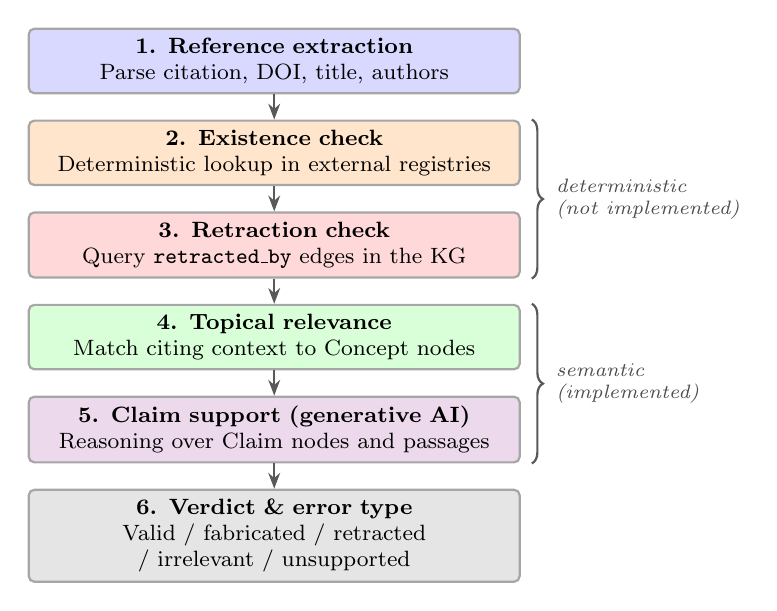
\begin{tikzpicture}[
  node distance=0.32cm,
  stepbox/.style={rectangle, rounded corners=2pt, draw=gray!70, thick, minimum width=6.2cm, minimum height=0.75cm, align=center, font=\footnotesize, text width=6cm},
  arr/.style={-{Stealth[length=2mm]}, thick, draw=gray!70!black},
  lab/.style={font=\scriptsize\itshape, text=gray!60!black, align=left}
]
\node[stepbox, fill=blue!15] (s1) {\textbf{1. Reference extraction}\\ Parse citation, DOI, title, authors};
\node[stepbox, fill=orange!20, below=of s1] (s2) {\textbf{2. Existence check}\\ Deterministic lookup in external registries};
\node[stepbox, fill=red!15, below=of s2] (s3) {\textbf{3. Retraction check}\\ Query \texttt{retracted\_by} edges in the KG};
\node[stepbox, fill=green!15, below=of s3] (s4) {\textbf{4. Topical relevance}\\ Match citing context to Concept nodes};
\node[stepbox, fill=violet!15, below=of s4] (s5) {\textbf{5. Claim support (generative AI)}\\ Reasoning over Claim nodes and passages};
\node[stepbox, fill=gray!20, below=of s5] (s6) {\textbf{6. Verdict \& error type}\\ Valid / fabricated / retracted / irrelevant / unsupported};
\draw[arr] (s1) -- (s2);
\draw[arr] (s2) -- (s3);
\draw[arr] (s3) -- (s4);
\draw[arr] (s4) -- (s5);
\draw[arr] (s5) -- (s6);
\draw[decorate, decoration={brace, amplitude=4pt}, thick, draw=gray!70!black]
  ([xshift=4pt]s2.north east) -- ([xshift=4pt]s3.south east)
  node[midway, right=5pt, lab] {deterministic\\(not implemented)};
\draw[decorate, decoration={brace, amplitude=4pt}, thick, draw=gray!70!black]
  ([xshift=4pt]s4.north east) -- ([xshift=4pt]s5.south east)
  node[midway, right=5pt, lab] {semantic\\(implemented)};
\end{tikzpicture}
}
\caption{Target verification workflow for one citation context. Stages 1, 4 and 5 are covered by the implementation reported in this article; stages 2, 3 and 6 are future work.}
\label{fig:target_workflow}
\end{figure}

\subsection{Design versus implementation}

The initial design of the pipeline assumed a dedicated stack (a bibliographic PDF parser, a property-graph database with graph embeddings, external bibliographic registries and both an open and a proprietary LLM). The implementation instead instantiates the design inside LightRAG, an open GraphRAG framework, which fixed the parser, the storage model and the retrieval procedure. Table~\ref{tab:design_vs_impl} lists the differences; each of them is revisited in Section~\ref{sec:discussion}.

\begin{table}[!t]
\centering
\footnotesize
\caption{Target design versus the implementation reported here.}
\label{tab:design_vs_impl}
\begin{tabular}{p{1.9cm} p{2.6cm} p{3.1cm}}
\toprule
Component & Target design & Implemented \\
\midrule
PDF parsing & GROBID (sections, markers, bibliography) & LightRAG legacy text extraction, no structure \\
Citation context & citing sentence $\pm$1 sentence & chunk-level extraction; the citing sentence is stored on the \texttt{cites} edge \\
KG schema & Paper, Author, Venue, Concept, Claim, CitationContext; \texttt{cites}, \texttt{supports}, \texttt{contradicts}, \texttt{retracted\_by}, \texttt{about\_topic} & nine types (Table~\ref{tab:entity_types}) and fourteen relations (Table~\ref{tab:relation_types}); no retraction edges \\
External linking & OpenAlex, Wikidata, Crossref & none; identifiers extracted as nodes only \\
Graph store & Neo4j, Cypher, Graph Data Science & NetworkX graph persisted as GraphML, undirected edges \\
Graph embeddings & node2vec, TransE, GNN & none; name-based entity lookup \\
LLMs & Llama~3.1~70B and GPT-4o & Claude Opus 5.5 through the Claude Agent SDK \\
Retrieval & two-hop evidence subgraph & keyword $\rightarrow$ entity lookup, one-hop edge expansion, weighted chunk selection \\
Scoring & logistic fusion of three signals with temperature scaling & single LLM label with rationale and evidence identifiers \\
Evaluation & expert gold standard, baselines, human study & descriptive statistics, schema audit, label coverage, \pilotN-pair pilot without gold labels \\
Hardware & four A100 GPUs & laptop CPU; the LLM is served remotely \\
\bottomrule
\end{tabular}
\end{table}

\section{The Implemented System}
\label{sec:system}

\subsection{Pipeline overview}

Figure~\ref{fig:pipeline} summarizes the implemented pipeline. Documents are uploaded as PDF files to the LightRAG server, converted to plain text, split into overlapping chunks and passed to the LLM with a schema-guided extraction prompt. Extracted entities and relations are merged by name across chunks, their descriptions are summarized by the LLM when they grow long, and the result is persisted as a NetworkX graph plus JSON key--value stores for chunks, document status and the LLM response cache. At query time the LLM extracts keywords from the question, the keywords are matched to entity names in the graph, the matched entities are expanded to their edges, the chunks referenced by those entities and edges are selected, and the assembled context is passed to the LLM. The verification prompt of Section~\ref{sec:verifier} consumes the same context.

\begin{figure}[!t]
\centering
\resizebox{0.9\columnwidth}{!}{
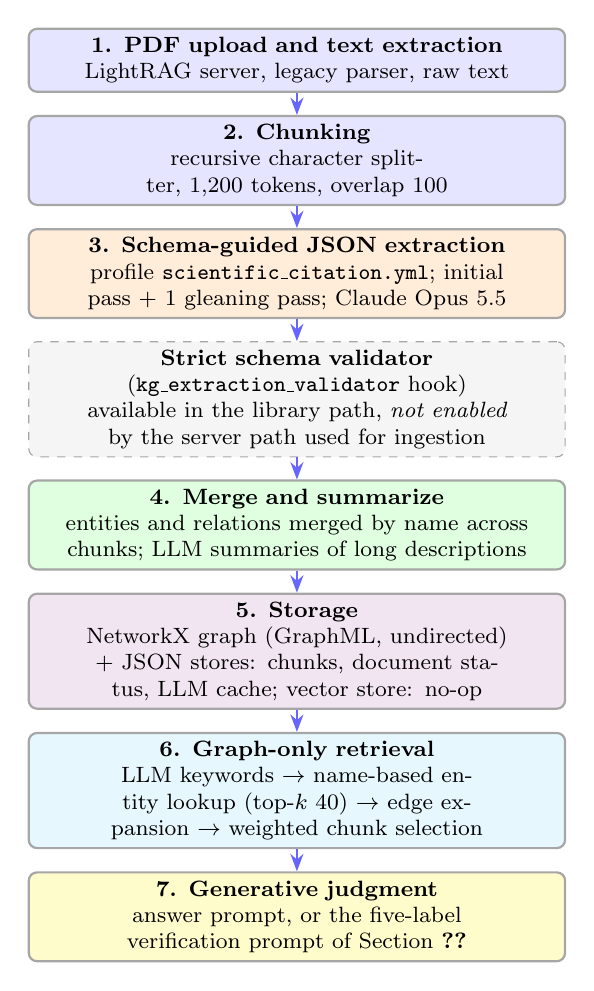
\begin{tikzpicture}[
  node distance=0.28cm,
  stage/.style={rectangle, rounded corners=3pt, draw=gray!70, thick, text width=6.6cm, align=center, minimum height=0.8cm, font=\footnotesize, inner sep=3pt},
  side/.style={rectangle, rounded corners=3pt, draw=gray!70, dashed, text width=6.6cm, align=center, minimum height=0.6cm, font=\footnotesize, inner sep=3pt, fill=gray!8},
  arr/.style={-{Stealth[length=2.2mm]}, thick, blue!60}
]
\node[stage, fill=blue!10] (s1) {\textbf{1. PDF upload and text extraction}\\ LightRAG server, legacy parser, raw text};
\node[stage, fill=blue!10, below=of s1] (s2) {\textbf{2. Chunking}\\ recursive character splitter, \chunkSize{} tokens, overlap \chunkOverlap};
\node[stage, fill=orange!15, below=of s2] (s3) {\textbf{3. Schema-guided JSON extraction}\\ profile \texttt{scientific\_citation.yml}; initial pass + \maxGleaning{} gleaning pass; Claude Opus 5.5};
\node[side, below=of s3] (s3b) {\textbf{Strict schema validator} (\texttt{kg\_extraction\_validator} hook)\\ available in the library path, \emph{not enabled} by the server path used for ingestion};
\node[stage, fill=green!12, below=of s3b] (s4) {\textbf{4. Merge and summarize}\\ entities and relations merged by name across chunks; LLM summaries of long descriptions};
\node[stage, fill=violet!10, below=of s4] (s5) {\textbf{5. Storage}\\ NetworkX graph (GraphML, undirected) + JSON stores: chunks, document status, LLM cache; vector store: no-op};
\node[stage, fill=cyan!10, below=of s5] (s6) {\textbf{6. Graph-only retrieval}\\ LLM keywords $\rightarrow$ name-based entity lookup (top-$k$ \topK) $\rightarrow$ edge expansion $\rightarrow$ weighted chunk selection};
\node[stage, fill=yellow!20, below=of s6] (s7) {\textbf{7. Generative judgment}\\ answer prompt, or the five-label verification prompt of Section~\ref{sec:verifier}};
\draw[arr] (s1) -- (s2);
\draw[arr] (s2) -- (s3);
\draw[arr] (s3) -- (s3b);
\draw[arr] (s3b) -- (s4);
\draw[arr] (s4) -- (s5);
\draw[arr] (s5) -- (s6);
\draw[arr] (s6) -- (s7);
\end{tikzpicture}
}
\caption{The implemented pipeline. Stages 1--5 run at ingestion, stages 6--7 at query time. The dashed stage exists in the code base but was not active during the ingestion reported here.}
\label{fig:pipeline}
\end{figure}

\subsection{Citation-oriented extraction schema}
\label{sec:schema}

LightRAG extracts entities and relations with a generic prompt in which the entity types are free-text guidance and the relation keywords are free text. The schema of this work is injected through that guidance slot as a versioned prompt profile. It declares nine entity types, \emph{Paper}, \emph{Author}, \emph{Organization}, \emph{Venue}, \emph{Identifier}, \emph{Methodology}, \emph{Dataset}, \emph{Concept} and \emph{Claim}, with \emph{Other} as fallback, and a controlled vocabulary of fourteen relation keywords: \texttt{cites}, \texttt{supports}, \texttt{contradicts}, \texttt{authored\_by}, \texttt{affiliated\_with}, \texttt{published\_in}, \texttt{has\_identifier}, \texttt{proposes}, \texttt{uses\_method}, \texttt{uses\_dataset}, \texttt{extends}, \texttt{compares\_with}, \texttt{addresses} and \texttt{related\_to}. The keyword field of every relation must start with exactly one vocabulary verb, optionally followed by free secondary keywords.

Four domain rules turn this schema into a citation graph. First, every bibliography entry yields one \emph{Paper} node plus its \emph{Author}, \emph{Venue} and \emph{Identifier} nodes; identifiers are stored as bare lower-case DOIs or arXiv identifiers. Second, an in-text marker such as ``[12]'' or ``(Smith et al., 2020)'' refers to a cited \emph{Paper} and must be resolved to the name used for the bibliography entry whenever both are visible. Third, when a sentence makes a statement and cites one or more papers for it, the model creates a \emph{Claim} node for the statement, links the citing \emph{Paper} to each cited \emph{Paper} with \texttt{cites}, stores the full citing sentence in the description of that edge, and links each cited \emph{Paper} to the \emph{Claim} with \texttt{supports}. Fourth, the article being read is itself a \emph{Paper} node named by its title or, when the title is not visible in the chunk, by the generic label ``This Paper''. The fourth rule has a measurable side effect that Section~\ref{sec:citation_structure} quantifies.

\subsection{Extraction, gleaning and validation}

Extraction runs in JSON mode: for each chunk the model returns a JSON object with an \texttt{entities} list (name, type, description) and a \texttt{relationships} list (source, target, keywords, description). A second ``gleaning'' call asks the model for entities and relations it missed in the first pass, so every chunk costs two extraction calls. The framework lower-cases entity types and keeps relation keywords as free text; nothing in the core rejects an off-schema type or keyword.

Enforcement is therefore delegated to a validator hook that the framework calls on each chunk's extraction output before merging. The validator of this work drops entities whose every record carries a type outside the schema, drops relations whose keyword list contains no vocabulary verb, moves the vocabulary verb to the front of the keyword list, and drops relations whose endpoint was dropped (otherwise the merge would materialize the endpoint as an \textsc{unknown} node). The validator is unit-tested, but it is attached only in the library entry point; the corpus of this article was ingested through the REST server, which does not attach it. Section~\ref{sec:audit} measures what this omission cost by replaying the validator offline.

\subsection{Merging and graph storage}

Entities with the same name are merged across chunks into one node whose description concatenates the extracted descriptions, separated by a marker, and is rewritten by the LLM when the number of fragments or their length exceeds a threshold. Relations are merged per unordered pair of endpoints; their keyword lists are unioned and sorted alphabetically, so the ``vocabulary verb first'' convention of the profile does not survive merging and every analysis in this article tests keyword \emph{containment} rather than position. Each node and edge records the chunks and files it came from. The graph is persisted as an undirected NetworkX graph: the citing $\rightarrow$ cited direction exists only in the semantics of the keyword and in the order in which the endpoints were first written, a point that the retrieval and the pilot handle by convention (Section~\ref{sec:pilot}).

\subsection{Graph-only retrieval}
\label{sec:retrieval}

The default LightRAG retrieval embeds the keywords extracted from the question and searches vector indexes of entities, relations and chunks. During ingestion the embedding endpoint (a local bge-m3 model served on CPU) timed out repeatedly, so the vector store was replaced by a no-op implementation and the graph was built without any embedding. Querying such a workspace required a new lookup mode, \texttt{LABEL}, in which the low-level and high-level keywords returned by the LLM are split into terms and each term is matched against entity names by case-insensitive substring search with a simple score (exact match, prefix, then shorter names first, with a bonus at word boundaries); a multi-word term that matches nothing is retried word by word. Hits are merged round-robin across terms and capped at top-$k$ (\topK{} in this work). The matched entities are then expanded exactly as in the vector path: their edges are collected, ranked by node degree and edge weight, and the chunks referenced by the retained entities and edges are selected by weighted polling. Modes \texttt{local}, \texttt{global}, \texttt{hybrid} and \texttt{mix} work in this configuration; \texttt{naive} (pure vector search) cannot.

Auditing the server log for this article revealed that every query issued in this mode ended with a context of entities and relations but \emph{zero} source chunks. The two chunk-selection routines fall back from vector similarity to weighted polling only inside the branch that requires a chunk index, so with no index the method stayed ``vector'' and nothing was selected. The defect was fixed by forcing the weighted fallback whenever no chunk index is available, with regression tests for both routines. The fix post-dates the ingestion, which it does not affect, and precedes the pilot of Section~\ref{sec:pilot}, whose contexts contain chunks.

\subsection{Generative verification module}
\label{sec:verifier}

The verification prompt receives the citing article, the citing sentence and the cited work, and asks for exactly one of five labels: \texttt{supports}, \texttt{partially\_supports}, \texttt{unrelated}, \texttt{contradicts} or \texttt{insufficient\_evidence}, the last one being an explicit abstention. The model must answer with a JSON object holding the label, a rationale of at most two sentences and the list of evidence identifiers (entity names, relation endpoints or chunk reference numbers) it relied on. Two conditions share this prompt. In the \emph{KG-grounded} condition the context assembled by the retrieval of Section~\ref{sec:retrieval} for the question ``Does the work $r$ support the statement $c$?'' is inserted as evidence and the system prompt forbids using anything else. In the \emph{LLM-only} condition no evidence is given and the model is told to rely on its own knowledge of the cited work. Because evidence identifiers are free text, the grounded condition can be audited mechanically: an identifier is counted as grounded only if it occurs verbatim in the retrieved context. The model, the effort setting and the decoding configuration are the same in both conditions and identical to those used at ingestion; the binding does not expose a temperature parameter.

\section{Experimental Setup}
\label{sec:setup}

\subsection{Corpus}

The corpus consists of \nPdfFiles{} PDF files uploaded to the server, of which \nPdfDistinct{} are distinct by content hash. The server queued \nDocsQueued{} documents and processed \nDocsProcessed{}; \nDocsFailedFont{} failed with a PDF font error in the text extractor and \nDocsFailedDup{} were rejected as byte-identical duplicates. Table~\ref{tab:corpus} lists the processed documents. They are open-access articles, conference papers, extended abstracts and one poster in computer science and engineering (vehicular networks, industrial machine learning, blockchain, forecasting, decision support, bibliometrics), almost all from one research group, which makes the corpus homogeneous in style and dense in self-citation rather than the multi-domain sample the target design calls for; \nShortDocs{} documents are one- or two-chunk extended abstracts or posters. Text extraction produced \nChars{} characters, chunked into \nChunks{} chunks of \meanTokensChunk{} tokens on average (\meanChunksDoc{} chunks per document).

% Generated by analysis/*.py -- do not edit by hand.
\begin{table*}[p]
\centering
\scriptsize
\caption{The 35 documents of the corpus after ingestion (venue and year as printed on the first page; dashes where the manuscript carries none). Chunks and tokens are those produced by the chunker; time is the per-document wall-clock span recorded in the document status store.}
\label{tab:corpus}
\begin{tabular}{l p{7.9cm} p{3.1cm} c r r r}
\toprule
ID & Title & Venue & Year & Chunks & Tokens & Time (s) \\
\midrule
D01 & A bibliometric analysis of feature selection techniques: trends, innovations, and future directions & IAES Int. J. of Artificial Intelligence & 2025 & 10 & 10,074 & 592 \\
D02 & A Comparative Study of Similarity Metrics for SVM-Based Recurrent Ticket Prediction (abstract) & ICRAMCS 2025 & 2025 & 1 & 857 & 199 \\
D03 & A Comprehensive Framework for Supplier Selection: Using Subjective, Objective, and Hybrid Multi-Criteria Decision-Making Techniques With Sensitivity Analysis & IEEE Access & 2024 & 17 & 18,583 & 937 \\
D04 & A Deep Learning Pipeline for Accurate Road Detection in Satellite Imagery & Int. J. of Engineering & 2026 & 15 & 13,924 & 799 \\
D05 & A Hybrid Approach for Sales Forecasting: Combining Deep Learning and Time Series Analysis & Int. J. of Engineering & 2025 & 17 & 15,889 & 793 \\
D06 & A Hybrid Probabilistic Modeling Approach to Analyzing Overstock Risk in Inventory Management: Integrating Bayesian Network Inference with Fuzzy Logic (abstract) & M3A 2024 & 2024 & 1 & 863 & 170 \\
D07 & Accurate AI Assistance in Contract Law Using Retrieval-Augmented Generation to Advance Legal Technology & IJACSA & 2025 & 14 & 13,803 & 351 \\
D08 & An overview of the Security Improvements of Artificial Intelligence in MANET & --- & --- & 7 & 8,092 & 436 \\
D09 & Application of Serial Temporal Deep Learning Models in Statistical Control Chart for Process Stability Monitoring: A Case Study in Injection Molding Manufacturing (abstract) & M3A 2024 & 2024 & 1 & 777 & 147 \\
D10 & Assessing Musculoskeletal Disorder Susceptibility in Professional Drivers Using K-Means Algorithms & Informatica & 2025 & 12 & 10,911 & 640 \\
D11 & Burnout: A Pervasive Challenge Threatening Workplace Well-Being and Organizational Success & Int. J. of Professional Business Review & 2024 & 16 & 14,074 & 613 \\
D12 & Comparative studies of the SARIMA and LSTM models for sales forecasting of a product category in a Marketplace (abstract) & ICRAMCS 2022 & 2022 & 1 & 707 & 92 \\
D13 & Configuration Driven Performance Analysis of Hyperledger Fabric: An Empirical Study & IEEE Access (manuscript) & --- & 23 & 26,227 & 766 \\
D14 & Decentralized Authentication Mechanism for Mobile Ad hoc Networks & Infocommunications Journal & 2022 & 22 & 25,037 & 144 \\
D15 & Design of Combined AHP-TOPSIS Model for Optimizing Selection of Injection Molding Machines & Int. J. of Engineering & 2025 & 18 & 18,330 & 945 \\
D16 & Development of a Blockchain Solution for Vehicle Management within a Consortium using Hyperledger Fabric (poster) & --- & --- & 2 & 1,402 & 200 \\
D17 & Enhancing Predictive Analysis of Vehicle Accident Risk: A Fuzzy-Bayesian Approach & IJACSA & 2024 & 21 & 20,124 & 576 \\
D18 & Explainable machine learning models applied to predicting customer churn for e-commerce & IAES Int. J. of Artificial Intelligence & 2025 & 13 & 12,654 & 705 \\
D19 & Feature Selection and Classification Performance: A Multi-Dataset Comparative Analysis Using Boruta Algorithm and Random Forest & EECSS'24 (CIST) & 2024 & 8 & 6,110 & 428 \\
D20 & From Uncertainty to Decision: An Intelligent Predictive Maintenance Approach Leveraging Fuzzy Bayesian Networks for Critical IT Components & IEEE Access (manuscript) & --- & 19 & 20,454 & 818 \\
D21 & Generative Adversarial Networks: A Systematic Review of Characteristics, Applications, and Challenges in Financial Data Generation and Market Modeling: 2019-2024 & Int. J. of Engineering & 2026 & 16 & 16,358 & 793 \\
D22 & Harnessing multi-source data for AI-Driven oncology insights: Productivity, trend, and sentiment analysis & Applied Computer Science & 2025 & 13 & 13,536 & 813 \\
D23 & Hybrid Approach Integrating Deep Learning-Autoencoder With Statistical Process Control Chart for Anomaly Detection: Case Study in Injection Molding Process & IEEE Access & 2024 & 21 & 23,228 & 1,101 \\
D24 & Implementation of Digital Twin and Deep Learning for Process Monitoring: Case Study in Injection Molding Manufacturing & EECSS'24 (CIST) & 2024 & 8 & 6,046 & 428 \\
D25 & Integrating Canny Filter and Convolutional Neural Networks for Quality Defect Detection in Injection Molding Process & EECSS'24 (MVML) & 2024 & 9 & 7,735 & 469 \\
D26 & Machine Learning for Industrial Manufacturing: A Case Study on Injection Molding Machine Selection Support & Springer proceedings (DATA 2024) & 2024 & 4 & 4,646 & 1 \\
D27 & Machine learning-assisted decision support in industrial manufacturing: a case study on injection molding machine selection & IAES Int. J. of Artificial Intelligence & 2025 & 17 & 15,634 & 595 \\
D28 & Microservices-Driven Automation in Full-Stack Development: Bridging Efficiency and Innovation with FSMicroGenerator & IEEE Access (manuscript) & --- & 27 & 30,862 & 944 \\
D29 & Review in Authentication for Mobile Ad hoc Network & --- & --- & 5 & 4,926 & 324 \\
D30 & Specification-Driven Synthetic Tabular Data Generation for System Validation and Management Decision Support & J. of Logistics Informatics and Service Science & 2026 & 15 & 14,306 & 699 \\
D31 & Symbiotic Combination of a Bayesian Network and Fuzzy Logic to Quantify the QoS in a VANET: Application in Logistic 4.0 & Computers & 2023 & 12 & 13,164 & 545 \\
D32 & The evolution and impact of artificial intelligence in market analysis: A quantitative bibliometric exploration of the past thirty-five (35) years & Applied Computer Science & 2025 & 12 & 10,372 & 574 \\
D33 & The Potential of Artificial Intelligence in Human Resource Management & Applied Computer Science & 2024 & 11 & 10,451 & 612 \\
D34 & Toward Quantum-Safe Permissioned Blockchains: Evaluating Hybrid ML-DSA-65/ECDSA Signatures on Hyperledger Fabric & IEEE Access (manuscript) & --- & 43 & 48,602 & 1,071 \\
D35 & Using a Fuzzy-Bayesian Approach for Predicting the QoS in VANET & Applied Computer Systems & 2022 & 16 & 13,626 & 363 \\
\bottomrule
\end{tabular}
\par\smallskip\begin{minipage}{0.95\textwidth}\scriptsize Five further uploads failed: 2 with a PDF font error (\texttt{/DescendantFonts}) and 3 rejected as byte-identical duplicates of a document already queued.\end{minipage}
\end{table*}


\subsection{Configuration and environment}

Table~\ref{tab:config} gives the runtime configuration, read from the server environment file, the package defaults and the installed versions. The LLM is \texttt{\llmModel} accessed through the Claude Agent SDK with the operator's subscription login (no API key), with the ``\llmEffort'' effort setting, at most \maxAsync{} concurrent calls, a 240\,s timeout and three retries. The same model served extraction, summarization, keyword extraction and the pilot. Prompt caching of LLM responses is enabled, which makes re-runs reproducible but also means that an interrupted ingestion resumes from cached extractions. No random seed is fixed and the binding does not forward a temperature, so individual LLM outputs are not bit-reproducible; every count in this article is nevertheless recomputable from the stored artefacts by the accompanying scripts. The LightRAG fork with the citation profile, the validator and the \texttt{LABEL} lookup, the analysis scripts, the persisted graph, the LLM response cache, the pilot results and the annotation sheet are released together with this article.\footnote{Repository: \url{https://github.com/youssefelyaakoubi01/citation-kg-verification}.}

% Generated by analysis/*.py -- do not edit by hand.
\begin{table}[!t]
\centering
\footnotesize
\caption{Runtime configuration of the ingestion and query runs (values read from the server \texttt{.env}, the package defaults and the installed versions).}
\label{tab:config}
\begin{tabular}{p{3.0cm} p{4.9cm}}
\toprule
Parameter & Value \\
\midrule
Framework & LightRAG 1.5.8 (fork with the citation profile and the \texttt{LABEL} lookup) \\
Python / NetworkX & 3.14.4 / 3.6.1 \\
LLM binding & \texttt{claude\_agent\_sdk} (claude-agent-sdk 0.1.81, CLI 2.1.295) \\
LLM model / effort & \texttt{claude-opus-5-5} / medium \\
LLM concurrency / timeout / retries & 4 / 240~s / 3 \\
Parallel document inserts & 3 \\
Parser / chunker & legacy PDF text extraction / recursive character, 1200 tokens, overlap 100 \\
Extraction prompt & profile \texttt{scientific\_citation.yml}, JSON mode, 1 gleaning pass \\
Schema validator at ingestion & not enabled (server path) \\
Graph storage & \texttt{NetworkXStorage} (GraphML file) \\
KV and doc-status storage & \texttt{JsonKVStorage}, \texttt{JsonDocStatusStorage} \\
Vector storage / embeddings & \texttt{NoopVectorDBStorage} / none (bge-m3 endpoint configured but unused) \\
Entity lookup at query time & \texttt{LABEL} (name matching, no embeddings) \\
Retrieval budget & top-$k$ 40, chunk top-$k$ 20, 6,000 / 8,000 / 30,000 tokens (entities / relations / total) \\
Reranker & none \\
LLM response cache & true \\
Hardware & 11th Gen Intel(R) Core(TM) i5-1145G7 @ 2.60GHz, 8 threads, 15~GiB RAM, no GPU \\
\bottomrule
\end{tabular}
\end{table}


\subsection{Measures}

Five families of measures are reported, all computed offline from the stored artefacts except the pilot. \emph{Ingestion} measures come from the document status store, the LLM response cache and the server log (documents, chunks, tokens, LLM calls, sessions and wall-clock time). \emph{Graph} measures are computed with NetworkX on the persisted graph. \emph{Schema adherence} replays the strict validator over the cached extraction outputs. \emph{Label coverage} replays the name-based lookup for every cited work with three query formulations. The \emph{pilot} issues real retrieval and LLM calls for a sample of citation contexts. No accuracy, precision, recall or calibration figure is reported, because no annotated gold standard exists for this corpus; the pilot produces the annotation sheet from which one can be built. For the same reason no baseline is run: the bibliometric, embedding-similarity, LLM-only and KG-only baselines of the target design (Table~\ref{tab:design_vs_impl}) are only meaningful against gold labels. The LLM-only condition of the pilot is a point of comparison for the behaviour of the model, not a baseline for its accuracy. Uncertainty is reported as 95\% confidence intervals: Wilson score intervals for proportions over the sampled pairs and a percentile bootstrap (\pilotBootstrapResamples{} resamples, fixed seed) for Cohen's $\kappa$; each pilot condition was run once.

\section{Results}
\label{sec:results}

\subsection{Ingestion run}

Table~\ref{tab:ingestion} summarizes the run and Table~\ref{tab:sessions} its sessions. Ingestion took place on \ingestionDate{} in \nIngestionSessions{} server sessions totalling \ingestionWall{} of wall-clock time. The first session ended when the subscription session limit was reached (\nSessionLimitLines{} log lines report that error), and the remaining documents were processed in two later sessions after the server was restarted. \nAbortedSessions{} earlier sessions had run with the vector-store configuration (one test document, then two attempts aborted by embedding timeouts); \nCacheExtractReused{} of their cached extraction responses were reused by the final run. The cache holds \nCacheTotal{} LLM responses: \nCacheExtract{} extraction calls (exactly two per chunk), \nCacheSummary{} description summaries and \nCacheKeywords{} query keyword extractions. Per chunk the model emitted \meanEntitiesChunk{} entities and \meanRelationsChunk{} relations on average, \entitiesLogged{} entity mentions and \relationsLogged{} relation mentions in total, which the merge reduced to \nNodes{} nodes and \nEdges{} edges. Because documents are processed concurrently, the per-document spans recorded in the status store (mean \perDocWallMean\,s, maximum \perDocWallMax\,s) sum to \perDocWallSum{}, more than the wall-clock time.

% Generated by analysis/*.py -- do not edit by hand.
\begin{table}[!t]
\centering
\footnotesize
\caption{Ingestion run: inputs, LLM calls, extraction volume and wall-clock time (from the document status store, the LLM response cache and the server log).}
\label{tab:ingestion}
\begin{tabular}{p{5.0cm} r}
\toprule
Measure & Value \\
\midrule
PDF files uploaded / distinct by hash & 59 / 37 \\
Documents queued / processed / failed & 40 / 35 / 5 \\
Text chunks (1\,200 tokens, overlap 100) & 467 \\
Tokens chunked (mean / max per chunk) & 472,384 (1,012 / 1,196) \\
Cached LLM calls: extraction / summary / keywords & 934 / 376 / 8 \\
Extraction calls per chunk & 2.0 \\
Entities / relations emitted per chunk (mean) & 41.7 / 52.3 \\
Entity mentions / relation mentions before merging & 19,502 / 24,463 \\
Distinct entity names / relation pairs per document (sum) & 14,667 / 21,528 \\
Nodes / edges after merging & 12,309 / 20,537 \\
Ingestion sessions (server restarts) & 3 \\
Ingestion wall-clock (sum of sessions) & 2~h 18~min \\
Per-document span: mean / median / max & 562~s / 592~s / 1,101~s \\
Aborted attempts before the run (wall-clock) & 3 (26~min 10~s) \\
Extraction responses reused from those attempts & 38 \\
Log lines reporting the subscription session limit & 46 \\
\bottomrule
\end{tabular}
\end{table}

% Generated by analysis/*.py -- do not edit by hand.
\begin{table}[!t]
\centering
\scriptsize
\caption{Server sessions that extracted chunks, from the log timestamps (a session ends at a restart or after ten idle minutes). Aborted sessions used the vector-store configuration that was later abandoned; their cached extractions were reused.}
\label{tab:sessions}
\begin{tabular}{l l l r r r l}
\toprule
\# & Start & End & Duration & Chunks & Docs & Kind \\
\midrule
1 & 2026-10-07 22:54 & 22:54 & 7~s & 1 & 0 & aborted \\
2 & 2026-10-08 00:07 & 00:30 & 23~min 12~s & 88 & 0 & aborted \\
3 & 2026-10-08 00:46 & 00:49 & 2~min 51~s & 17 & 0 & aborted \\
4 & 2026-10-08 00:55 & 02:32 & 1~h 36~min & 343 & 24 & ingestion \\
5 & 2026-10-08 13:38 & 13:54 & 15~min 50~s & 85 & 4 & ingestion \\
6 & 2026-10-08 23:04 & 23:31 & 27~min 02~s & 114 & 7 & ingestion \\
\bottomrule
\end{tabular}
\end{table}


\subsection{Graph statistics}

Table~\ref{tab:graph_summary} describes the merged graph: \nNodes{} nodes and \nEdges{} undirected edges, a density of \graphDensity{}, a mean degree of \meanDegree{}, \nComponents{} connected components of which the giant one holds \giantComponent{} nodes, and \nIsolated{} isolated nodes. Tables~\ref{tab:entity_types} and~\ref{tab:relation_types} and Figs.~\ref{fig:entity_types} and~\ref{fig:relation_types} give the type distributions. \emph{Author} (\nAuthorNodes) and \emph{Paper} (\nPaperNodes) are the largest classes, followed by \emph{Concept}, \emph{Methodology} and \emph{Claim} (\nClaimNodes); only \nUnknownNodes{} nodes carry the \textsc{unknown} type that the merge assigns to relation endpoints never extracted as entities. Every edge contains at least one vocabulary keyword, and \nEdgesMultiVocab{} edges contain more than one because they merged extractions with different verbs. The most frequent relations are \texttt{related\_to} (\nRelatedToEdges), \texttt{addresses} (\nAddressesEdges) and \texttt{authored\_by} (\nAuthoredByEdges); the citation relations \texttt{cites} and \texttt{supports} account for \nCitesEdges{} and \nSupportsEdges{} edges, and \texttt{contradicts} for \nContradictsEdges{}. The degree distribution (Fig.~\ref{fig:degree_loglog}) is heavy-tailed, with one outlier at degree \maxDegree{}: the generic ``This Paper'' node, which merged the citing article of \hubFiles{} documents whose title was not visible in the chunk being processed. Figure~\ref{fig:overview} shows the connected part of the subgraph produced by one document, and Fig.~\ref{fig:pyvis} the interactive rendering of the whole graph as it stood during ingestion.

% Generated by analysis/*.py -- do not edit by hand.
\begin{table}[!t]
\centering
\footnotesize
\caption{Size and shape of the merged knowledge graph.}
\label{tab:graph_summary}
\begin{tabular}{l r}
\toprule
Measure & Value \\
\midrule
Nodes & 12,309 \\
Edges (undirected) & 20,537 \\
Density & 2.71e-04 \\
Mean degree & 3.34 \\
Median degree & 1 \\
Maximum degree (``This Paper'') & 2,658 \\
Connected components & 55 \\
Giant component (nodes) & 12,087 \\
Isolated nodes & 12 \\
Entity types present & 11 \\
Edges with $\geq 1$ vocabulary keyword & 20,537 (100.0\%) \\
\bottomrule
\end{tabular}
\end{table}

% Generated by analysis/*.py -- do not edit by hand.
\begin{table}[!t]
\centering
\footnotesize
\caption{Nodes per entity type after merging. \textsc{unknown} nodes are relation endpoints that were never extracted as entities.}
\label{tab:entity_types}
\begin{tabular}{l r r}
\toprule
Type & Nodes & Share \\
\midrule
author & 2,804 & 22.8\% \\
paper & 2,290 & 18.6\% \\
concept & 1,980 & 16.1\% \\
methodology & 1,761 & 14.3\% \\
claim & 1,343 & 10.9\% \\
identifier & 872 & 7.1\% \\
venue & 801 & 6.5\% \\
organization & 208 & 1.7\% \\
dataset & 127 & 1.0\% \\
other & 121 & 1.0\% \\
\textsc{unknown} & 2 & 0.0\% \\
\bottomrule
\end{tabular}
\end{table}

% Generated by analysis/*.py -- do not edit by hand.
\begin{table}[!t]
\centering
\footnotesize
\caption{Edges whose keyword list contains each controlled relation keyword (an edge merged from several extractions can carry more than one).}
\label{tab:relation_types}
\begin{tabular}{l r r}
\toprule
Keyword & Edges & Share of edges \\
\midrule
\texttt{related\_to} & 4,197 & 20.4\% \\
\texttt{addresses} & 3,630 & 17.7\% \\
\texttt{authored\_by} & 3,423 & 16.7\% \\
\texttt{cites} & 2,296 & 11.2\% \\
\texttt{uses\_method} & 2,046 & 10.0\% \\
\texttt{supports} & 1,503 & 7.3\% \\
\texttt{published\_in} & 1,264 & 6.2\% \\
\texttt{has\_identifier} & 937 & 4.6\% \\
\texttt{proposes} & 659 & 3.2\% \\
\texttt{compares\_with} & 306 & 1.5\% \\
\texttt{extends} & 190 & 0.9\% \\
\texttt{affiliated\_with} & 178 & 0.9\% \\
\texttt{uses\_dataset} & 170 & 0.8\% \\
\texttt{contradicts} & 3 & 0.0\% \\
\bottomrule
\end{tabular}
\end{table}


\begin{figure}[!t]
\centering
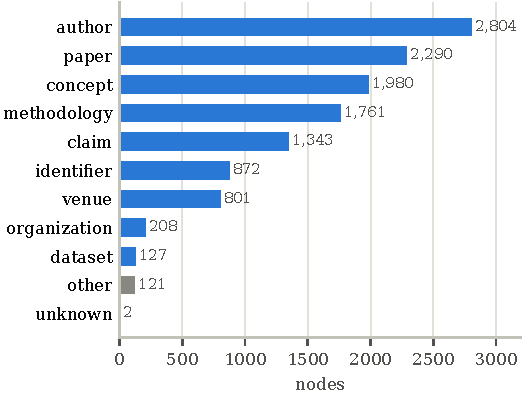
\includegraphics[width=\columnwidth]{fig_entity_types.pdf}
\caption{Nodes per entity type after merging (grey: the \emph{Other} fallback and the \textsc{unknown} endpoints).}
\label{fig:entity_types}
\end{figure}

\begin{figure}[!t]
\centering
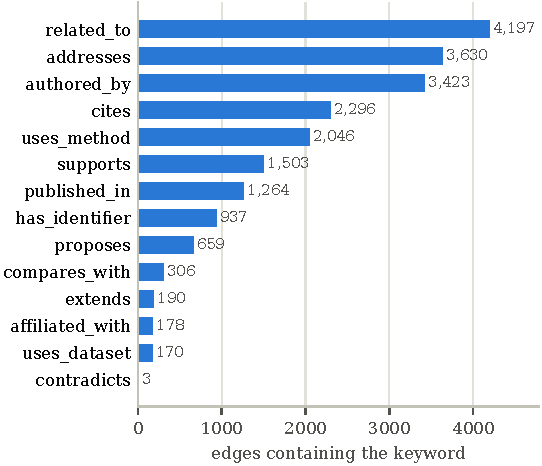
\includegraphics[width=\columnwidth]{fig_relation_types.pdf}
\caption{Edges containing each controlled relation keyword.}
\label{fig:relation_types}
\end{figure}

\begin{figure}[!t]
\centering
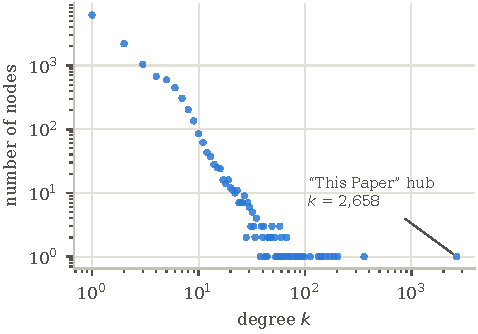
\includegraphics[width=\columnwidth]{fig_degree_loglog.pdf}
\caption{Degree distribution of the merged graph (log--log). The isolated point at the far right is the generic ``This Paper'' hub.}
\label{fig:degree_loglog}
\end{figure}

\begin{figure*}[!t]
\centering
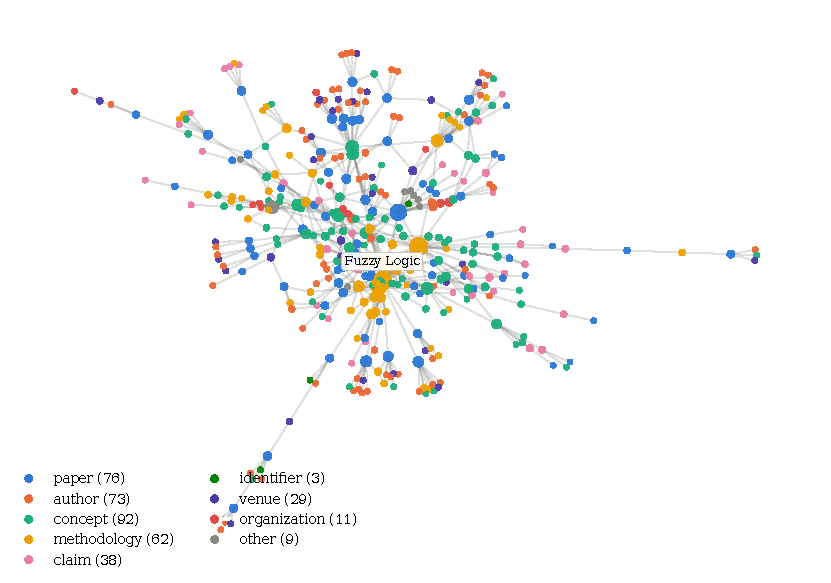
\includegraphics[width=0.9\textwidth]{fig_overview.pdf}
\caption{Largest connected component of the subgraph extracted from one document (Table~\ref{tab:corpus}, \emph{Symbiotic Combination of a Bayesian Network and Fuzzy Logic to Quantify the QoS in a VANET}): nodes coloured by type, sized by degree, spring layout with a fixed seed. The highest-degree node is labelled.}
\label{fig:overview}
\end{figure*}

\begin{figure*}[!t]
\centering
\subfloat[Whole graph]{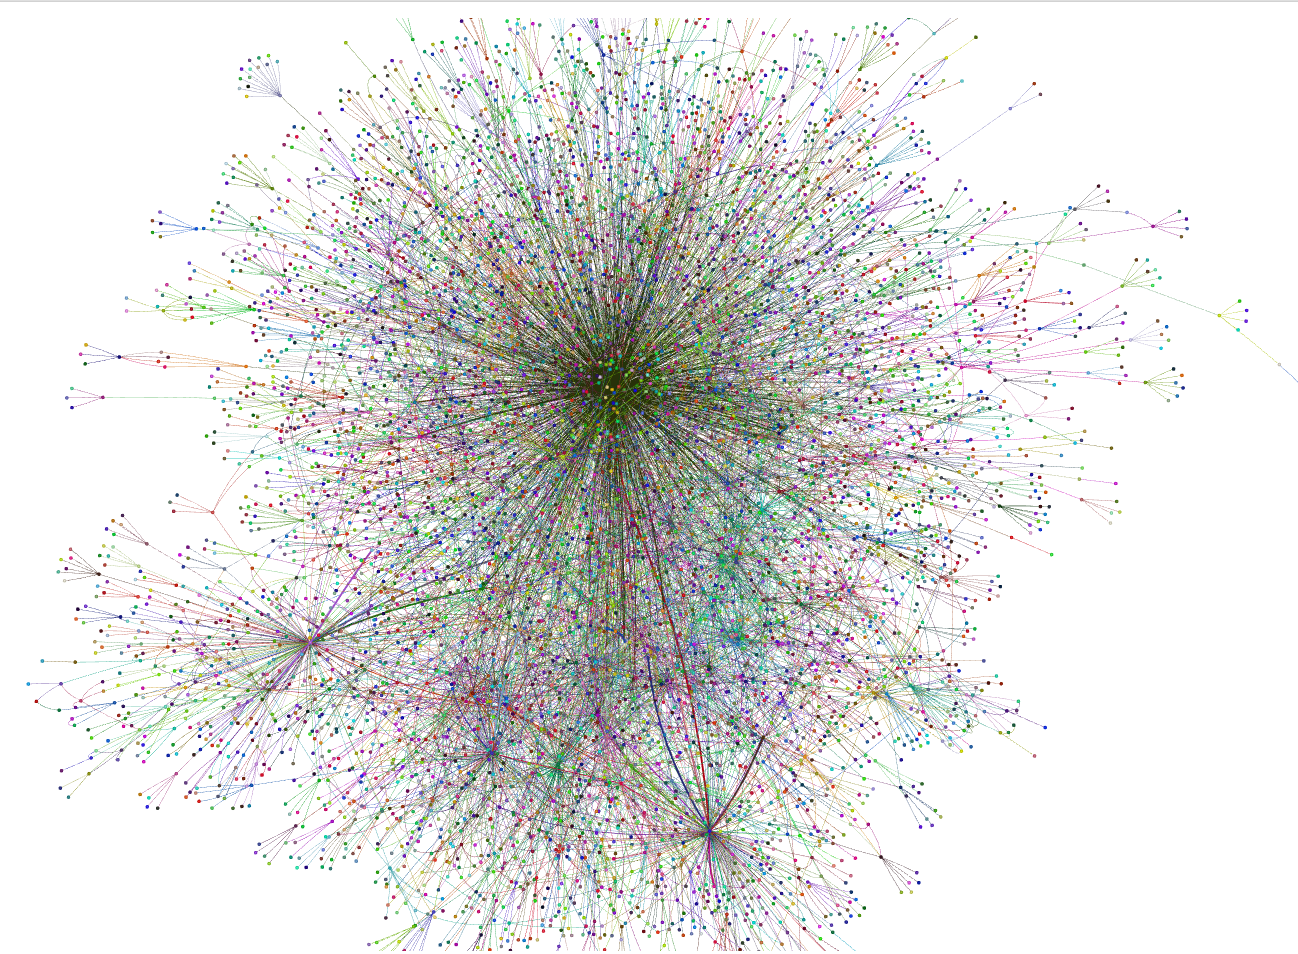
\includegraphics[width=0.46\textwidth]{pyvis_overview.png}}
\hfil
\subfloat[Zoom with node labels and a hovered edge description]{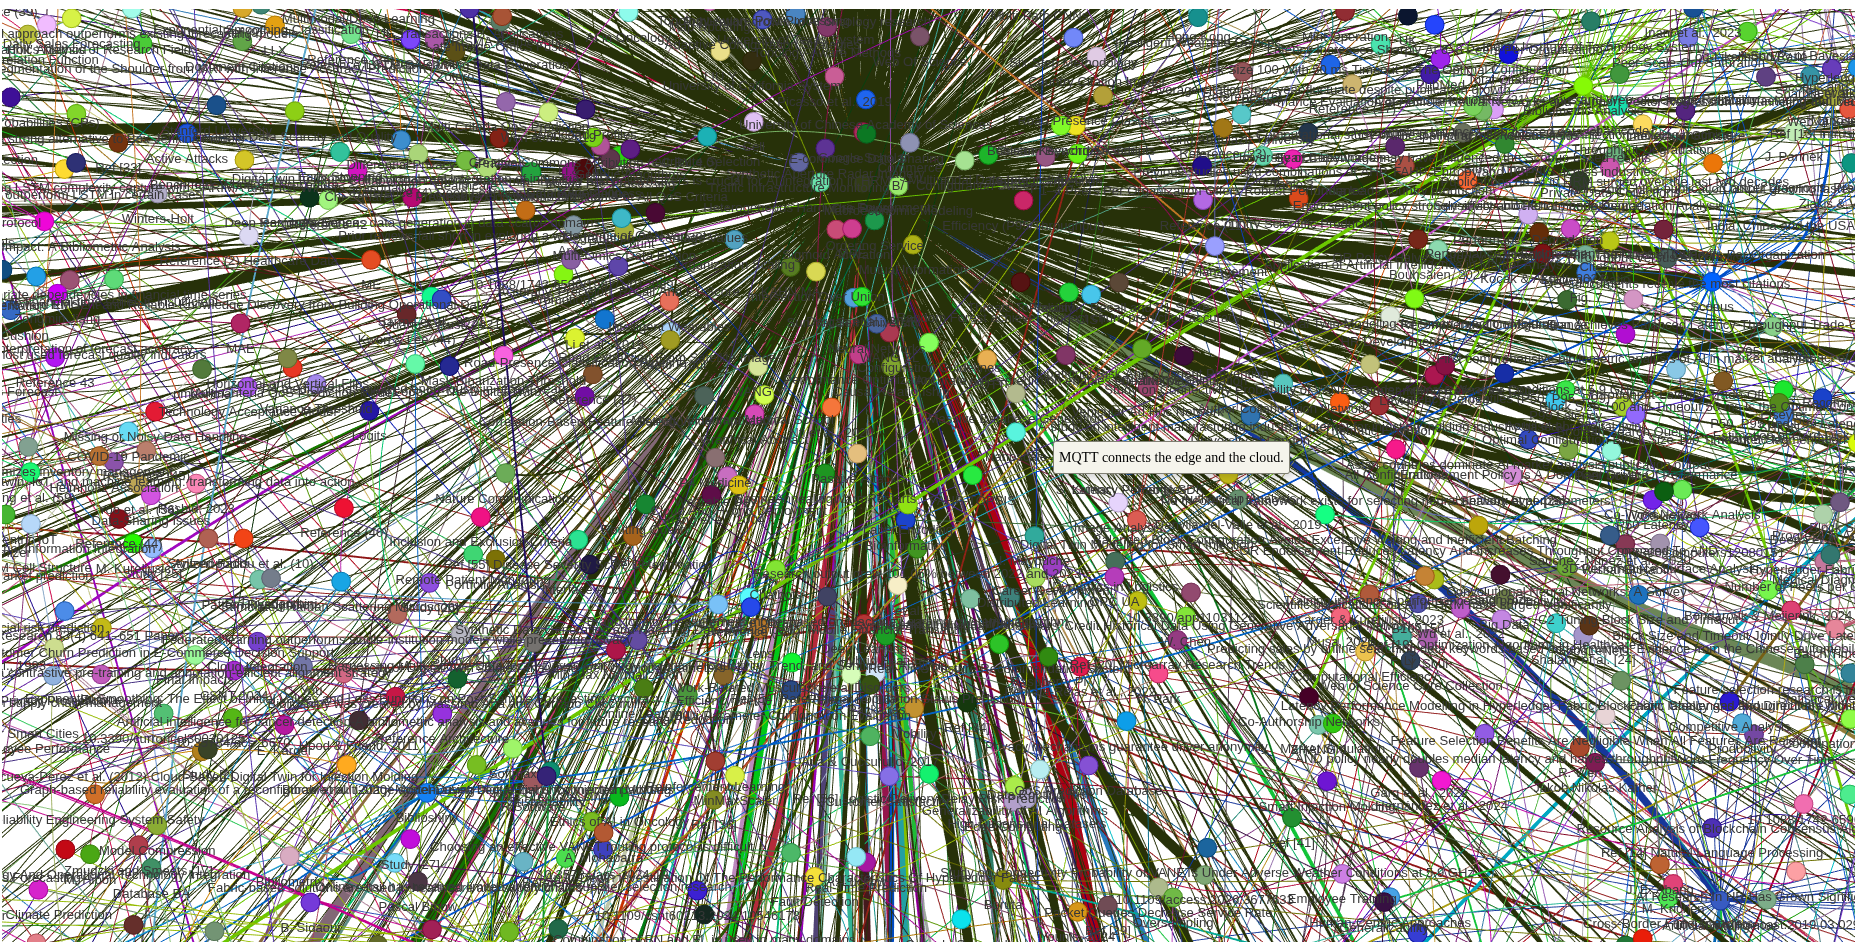
\includegraphics[width=0.46\textwidth]{pyvis_zoom.png}}
\caption{Interactive rendering of the knowledge graph (pyvis/vis-network, random node colours), captured during ingestion on 2026-10-08 when 24 of the \nDocsProcessed{} documents had been processed.}
\label{fig:pyvis}
\end{figure*}

\subsection{Schema adherence without enforcement}
\label{sec:audit}

Table~\ref{tab:schema_audit} reports the replay of the strict validator over the \auditRecords{} cached extraction responses (\auditChunks{} chunks, two passes each). All responses parsed as JSON (\auditRepaired{} needed automatic repair). None of the \auditEntities{} entity records carried a type outside the schema, and all \auditRelations{} relation records started with a vocabulary verb; the off-schema and no-vocabulary counts are zero in both passes. The initial pass emitted \auditEntPerInitial{} entities and \auditRelPerInitial{} relations per chunk, the gleaning pass \auditEntPerGleaning{} and \auditRelPerGleaning{}. The gleaning pass behaves differently in one respect: \pctGleanMissingSame{} of its relations name an endpoint that the same response does not list as an entity, because the entity was already listed in the initial pass. The framework merges both passes before invoking the validator, and on that merged view only \auditUnionPairsMissing{} relation pairs reference an endpoint absent from the chunk's entities (\auditUnknownTop); these are exactly the \nUnknownNodes{} \textsc{unknown} nodes of the final graph. Had the validator been enabled, it would have kept \pctEntKept{} of the entity records and \pctRelKept{} of the relation records. Prompt guidance alone therefore achieved complete schema adherence on this corpus with this model; the validator remains necessary as a guarantee, but it would have changed the graph by two edges.

% Generated by analysis/*.py -- do not edit by hand.
\begin{table*}[!t]
\centering
\scriptsize
\caption{Schema adherence of the raw extraction outputs, measured by replaying the strict validator over the cached LLM responses (the ingestion run itself did not enforce the schema). Initial pass and gleaning pass are reported separately.}
\label{tab:schema_audit}
\begin{tabular}{p{7.2cm} r r r}
\toprule
Measure & Initial pass & Gleaning pass & Both \\
\midrule
Cached responses & 467 & 467 & 934 \\
Responses needing JSON repair & 1 & 0 & 1 \\
Unparseable responses & 0 & 0 & 0 \\
Entity records emitted & 12,716 & 6,946 & 19,662 \\
\quad with a type outside the schema & 0 (0.0\%) & 0 (0.0\%) & 0 (0.0\%) \\
\quad with an invalid type string & 0 (0.0\%) & 0 (0.0\%) & 0 (0.0\%) \\
Distinct entity names per response (sum) & 12,716 & 6,946 & 19,662 \\
\quad dropped by the validator (all records off-schema) & 0 (0.0\%) & 0 (0.0\%) & 0 (0.0\%) \\
Relation records emitted & 14,419 & 10,115 & 24,534 \\
\quad keyword list starting with a vocabulary verb & 14,419 (100.0\%) & 10,115 (100.0\%) & 24,534 (100.0\%) \\
\quad with no vocabulary verb at all & 0 (0.0\%) & 0 (0.0\%) & 0 (0.0\%) \\
\quad whose endpoint is not listed in the same response & 2 (0.0\%) & 9,571 (94.6\%) & 9,573 (39.0\%) \\
\emph{Per chunk, both passes merged (as the validator would see them)} &  &  &  \\
Relation records &  &  & 24,534 \\
\quad with an endpoint absent from the chunk's entities &  &  & 2 (0.0\%) \\
\quad of which resolvable to an entity extracted in another chunk (pairs) &  &  & 0 \\
Entity records kept by the strict validator &  &  & 19,662 (100.0\%) \\
Relation records kept by the strict validator &  &  & 24,532 (100.0\%) \\
\bottomrule
\end{tabular}
\par\smallskip\begin{minipage}{0.95\textwidth}\scriptsize No off-schema entity type was emitted. Every relation carried at least one vocabulary verb.\end{minipage}
\end{table*}


\subsection{Citation structure}
\label{sec:citation_structure}

Table~\ref{tab:citation_coverage} isolates the part of the graph that matters for verification. The graph holds \nCites{} \texttt{cites} edges, \nCitesPaperPaper{} of them between two \emph{Paper} nodes, involving \nPapersInCites{} paper nodes and \nCitedResolved{} distinct cited works that resolve to a titled \emph{Paper} node. \nCitesSentenceStrict{} edges (\pctCitesSentenceStrict) quote the citing sentence or its bracketed marker in their description, and \nCitesSentence{} (\pctCitesSentence) carry at least a sentence-length context. On the claim side, \nSupports{} \texttt{supports} edges link \nCitedAndSupporting{} cited works to \emph{Claim} nodes; \nClaimsSupported{} of the \nClaims{} claims (\pctClaimsSupported) have at least one supporting paper and \nClaimsUnsupported{} have none. Combining the three conditions a verification needs, a quoted citing sentence, a resolved cited work and a claim supported by that work, leaves \nVerifiableEdges{} \texttt{cites} edges that can be verified end to end inside the graph. Figure~\ref{fig:ego_subgraph} shows such a structure for the citing paper with the most verifiable citations.

Two artefacts limit this coverage. First, \nCitesHub{} \texttt{cites} edges (\pctCitesHub) have the generic ``This Paper'' node as citing endpoint, so the citing article of those contexts can only be recovered from the file name recorded on the edge. Second, \nCitesPlaceholder{} \texttt{cites} edges (\pctCitesPlaceholder) end in one of \nPlaceholderNodes{} placeholder nodes named ``Reference [$n$]'' or ``[$n$]'': the bibliography entry was not visible in the chunk where the marker appeared, and the model, following the rule of Section~\ref{sec:schema}, kept the marker as a label. Partially resolved labels such as ``Ref [1] Hyperledger Fabric'' or ``Abbas et al. [9]'' (visible in Fig.~\ref{fig:ego_subgraph}) are a milder form of the same effect, and so are duplicate nodes for one work (``FIPS 204'' and ``NIST FIPS 204'' in the same figure), which the name-based merge cannot unify. Finally, only \nContradicts{} \texttt{contradicts} edges exist, which reflects both the corpus (articles rarely cite work they argue against) and a known tendency of extraction prompts to favour positive relations.

% Generated by analysis/*.py -- do not edit by hand.
\begin{table}[!t]
\centering
\footnotesize
\caption{Citation structure captured by the graph (counts over the merged graph).}
\label{tab:citation_coverage}
\begin{tabular}{p{4.9cm} r}
\toprule
Measure & Value \\
\midrule
\texttt{cites} edges & 2,296 \\
\quad between two \texttt{paper} nodes & 2,276 \\
\quad touching the ``This Paper'' hub & 1,378 \\
\quad with a placeholder endpoint (``Reference [$n$]'') & 497 \\
\quad quoting the citing sentence or its marker (strict) & 1,515 (66.0\%) \\
\quad with a sentence-length context ($\geq 8$ words, lenient) & 2,221 (96.7\%) \\
\texttt{paper} nodes in a \texttt{cites} edge & 1,971 \\
Distinct cited works (resolved \texttt{paper} nodes) & 1,755 \\
Placeholder nodes & 182 \\
\texttt{supports} edges & 1,503 \\
\quad \texttt{paper}$\rightarrow$\texttt{claim} & 1,494 \\
\texttt{claim} nodes & 1,343 \\
\quad with $\geq 1$ supporting paper & 1,098 (81.8\%) \\
\quad without any \texttt{supports} edge & 245 \\
Cited works that also support a claim & 652 \\
\texttt{cites} edges verifiable end to end (sentence + cited work + claim) & 328 \\
\texttt{contradicts} edges & 3 \\
\texttt{identifier} nodes / DOI-shaped & 872 / 849 \\
\bottomrule
\end{tabular}
\end{table}


\begin{figure*}[!t]
\centering
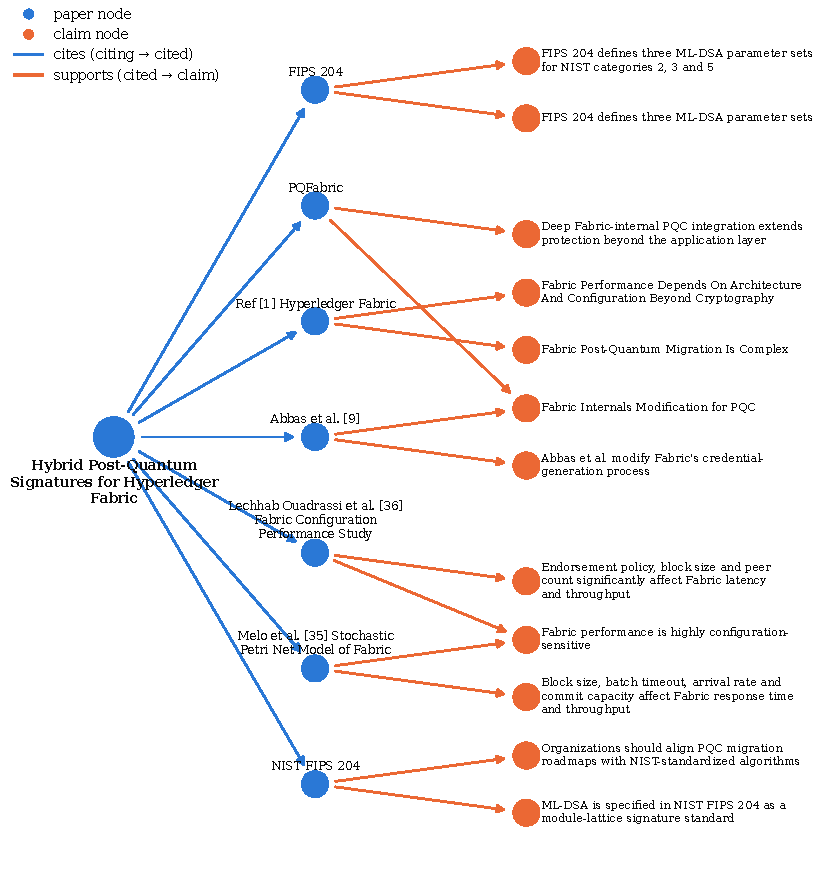
\includegraphics[width=0.95\textwidth]{fig_ego_subgraph.pdf}
\caption{Citing paper $\rightarrow$ cited paper $\rightarrow$ claim structure extracted for the citing paper with the most end-to-end verifiable citations (\emph{Hybrid Post-Quantum Signatures for Hyperledger Fabric}, an extraction label for document D34 of Table~\ref{tab:corpus}). Up to seven cited works and two claims per cited work are shown; every \texttt{cites} edge carries the citing sentence in its description.}
\label{fig:ego_subgraph}
\end{figure*}

\subsection{Resolving cited works at query time}
\label{sec:label}

Table~\ref{tab:label_coverage} measures whether the name-based lookup can bring a cited work into the context. For each of the \labelCitedWorks{} resolved cited works, the lookup was replayed with three formulations a verification query may carry. Queried with its full title, the work is the first entity returned in \labelFullTitleHitOne{} of cases and is within the top-$k$ in all of them; the misses at rank one come from titles that contain commas, which the keyword splitter treats as several terms. Queried with only the first three title tokens, the work is first in \labelPartialTitleHitOne{} of cases, within the top-$k$ in \labelPartialTitleHitForty{}, and reachable through the edge expansion in \labelPartialTitleReach{}. Queried with its first author, the lookup never returns the work itself (hit@1 \labelFirstAuthorHitOne) but always returns the author node, from which the work enters the context through its \texttt{authored\_by} edge (reach \labelFirstAuthorReach). The lookup therefore behaves as a lexical index: it is reliable when the query reproduces the stored name and degrades with paraphrase, which the keyword extraction step of the LLM must compensate for.

% Generated by analysis/*.py -- do not edit by hand.
\begin{table}[!t]
\centering
\scriptsize
\caption{Label-index resolution of the 1,755 distinct cited works: share recovered within the first $k$ entities returned by the name search used in \texttt{LABEL} lookup (top-$k$ = 40), for three query formulations a verification query may carry.}
\label{tab:label_coverage}
\begin{tabular}{l r r r r r r}
\toprule
Query & $n$ & hit@1 & hit@5 & hit@10 & hit@40 & reach \\
\midrule
full title & 1,755 & 95.3\% & 99.8\% & 99.9\% & 100.0\% & 100.0\% \\
partial title & 1,747 & 46.0\% & 71.8\% & 77.8\% & 88.7\% & 88.9\% \\
first author & 1,077 & 0.0\% & 9.6\% & 10.0\% & 11.2\% & 100.0\% \\
\bottomrule
\end{tabular}
\par\smallskip\begin{minipage}{0.95\columnwidth}\scriptsize ``partial title'': the first three title tokens of at least three characters. ``reach'': the cited work is itself among the returned entities or is adjacent to one of them, i.e. it enters the context through the edge expansion that follows the lookup. ``first author'' applies only to cited works linked to an \texttt{author} node; the search returns the author node, never the paper, so the work is reached through its \texttt{authored\_by} edge. Titles containing commas are split into several search terms by the keyword splitter.\end{minipage}
\end{table}


\subsection{Pilot: KG-grounded versus LLM-only judgments}
\label{sec:pilot}

Table~\ref{tab:pilot} reports the pilot. The sample consists of \pilotN{} \texttt{cites} edges from \pilotDocs{} documents, drawn at random with a fixed seed and at most three per document among the edges whose description quotes the citing sentence, whose cited work resolves to a titled \emph{Paper} node and whose cited work supports at least one \emph{Claim} node, that is, the end-to-end verifiable structures of Section~\ref{sec:citation_structure}. For each pair the question ``Does the work $r$ support the statement $c$?'' was submitted to the \texttt{hybrid} retrieval in \texttt{LABEL} mode, and the same model judged the pair once with the retrieved context (condition A) and once without it (condition B).

\textbf{Retrieval.} The retrieved context contained the cited work in \pilotCitedInCtxPct{} of the queries and at least one of its KG claims in \pilotClaimInCtxPct{}. On average it held \pilotEntitiesMean{} entities, \pilotRelationsMean{} relations and \pilotChunksMean{} chunks; \pilotChunksZero{} queries returned no chunk, which confirms that the repaired fallback of Section~\ref{sec:retrieval} was active. The citing sentence itself was found verbatim in a retrieved chunk for \pilotSentenceInChunksPct{} of the pairs. Once the keyword extraction of a question is cached, retrieval over the graph takes a median of \pilotRetMedian\,s; the uncached keyword extraction adds one LLM round trip. The grounded judgment took a median of \pilotAMedian\,s and the ungrounded one \pilotBMedian\,s.

\textbf{Labels and agreement.} With the graph, the model returned \texttt{supports} for \pilotASupportsPct{} of the pairs, \texttt{partially\_supports} for \pilotAPartiallySupportsPct{}, \texttt{unrelated} for \pilotAUnrelatedPct{} and abstained (\texttt{insufficient\_evidence}) for \pilotAInsufficientEvidencePct{}. Without the graph it abstained for \pilotBInsufficientEvidencePct{} of the pairs and returned \texttt{supports} for \pilotBSupportsPct{}. The two conditions agreed on \pilotAgreePct{} of the pairs (Cohen's $\kappa$ = \pilotKappa, 95\% bootstrap interval \pilotKappaCI); of the \pilotDisagree{} disagreements, \pilotBAbstainACommit{} are pairs on which the ungrounded model abstains while the grounded one commits to a label, and only \pilotAAbstainBCommit{} the reverse; both abstain on \pilotBothAbstain{} pairs. With \pilotN{} pairs the intervals are wide. The Wilson intervals of the two abstention rates, \pilotAInsufficientEvidenceCI{} with the graph and \pilotBInsufficientEvidenceCI{} without it, do not overlap, whereas the interval of $\kappa$ includes zero: the conditions differ in how often they abstain, but their label agreement cannot be distinguished from chance at this sample size. Neither distribution can be read as accuracy: the annotation sheet produced by the pilot (one row per pair with both judgments and rationales) is the material from which correctness will be established.

\textbf{Grounding.} \pilotAEvidencePct{} of the grounded answers listed evidence identifiers, against \pilotBEvidencePct{} of the ungrounded ones, and \pilotIdsGroundedPct{} (95\% interval \pilotIdsGroundedCI) of the \pilotIdsTotal{} identifiers cited by the grounded answers occur verbatim in the retrieved context. The grounded rationales can therefore be audited mechanically down to the entity, relation or chunk they rest on, which is the property the target design requires of an explanation.

\textbf{Reading the rationales.} \pilotMarkerPairs{} of the \pilotN{} sampled cited works carry a marker-derived label such as ``Study [14] Bayesian Networks'' rather than a title. On those pairs the ungrounded model abstains \pilotMarkerBAbstain{} times, because the label does not identify a work it could know, whereas the grounded model commits to a label \pilotMarkerACommit{} times and abstains \pilotMarkerAAbstain{} times; its rationales commit when the retrieved descriptions include the bibliography entry (authors, year, title) or the citing article's account of the cited finding, and abstain when the only evidence is the citing sentence restated as an entity description. On the \pilotTitledPairs{} pairs whose cited work has a title, the two conditions abstain equally often (\pilotTitledAAbstain{} and \pilotTitledBAbstain{} times). This exposes a circularity that the graph alone cannot remove: most evidence about a cited work comes from the citing article (its bibliography entry, its own restatement of the cited finding), so a \texttt{supports} label often means that the citing article's account of the cited work is consistent with its citing sentence, not that the cited text was checked. Closing that gap requires the cited full texts in the graph, which is the first item of future work.

% Generated by analysis/*.py -- do not edit by hand.
\begin{table}[!t]
\centering
\scriptsize
\caption{Pilot on 50 citation contexts: KG-grounded (A) versus LLM-only (B) claim-support judgments by the same model. No gold labels exist, so the table reports distributions, agreement, retrieval coverage and verifiable grounding, not accuracy. Brackets give 95\% confidence intervals in percent.}
\label{tab:pilot}
\begin{tabular}{@{}p{3.3cm} r r@{}}
\toprule
Measure & A: KG-grounded & B: LLM-only \\
\midrule
Pairs (documents) & 50 (22) &  \\
\emph{Label distribution} & KG-grounded (A) & LLM-only (B) \\
\hspace{2pt}\texttt{supports} & 18 (36.0\%) [24--50] & 15 (30.0\%) [19--44] \\
\hspace{2pt}\texttt{partially\_supports} & 13 (26.0\%) [16--40] & 2 (4.0\%) [1--13] \\
\hspace{2pt}\texttt{unrelated} & 1 (2.0\%) [0--10] & 1 (2.0\%) [0--10] \\
\hspace{2pt}\texttt{insufficient\_evidence} & 18 (36.0\%) [24--50] & 32 (64.0\%) [50--76] \\
Agreement A = B & 23 (46.0\%) [33--60] &  \\
Cohen's $\kappa$ [bootstrap CI] & 0.17 [-0.02, 0.36] &  \\
\emph{Retrieval (condition A)} &  &  \\
Entities / relations / chunks per query (mean) & 68.3 / 157.1 / 14.3 &  \\
Queries with zero chunks & 0 &  \\
Cited work present in the context & 50 (100.0\%) &  \\
A KG claim of the cited work present & 41 (82.0\%) [69--90] &  \\
Citing sentence found in a retrieved chunk & 7 (14.0\%) [7--26] &  \\
\emph{Grounding of the answer} & A & B \\
Answers listing evidence identifiers & 50 (100.0\%) & 0 (0.0\%) \\
Identifiers that occur verbatim in the context & 175 / 187 (93.6\%) [89--96] & n/a \\
\emph{Latency (median)} &  &  \\
Retrieval / judgment A / judgment B & 0.2~s / 6.3~s & 4.3~s \\
\bottomrule
\end{tabular}
\par\smallskip\begin{minipage}{0.95\columnwidth}\scriptsize Intervals: Wilson score for proportions over the 50 pairs (or over the identifiers); percentile bootstrap (10,000 resamples, fixed seed) for $\kappa$. Each condition was run once, so the intervals reflect sampling of pairs, not the run-to-run variation of the model.\end{minipage}
\end{table}


\section{Discussion}
\label{sec:discussion}

\subsection{Answers to the research questions}

\textbf{RQ1.} A schema-guided extraction inside a general-purpose GraphRAG framework did build a citation graph from raw PDFs: \nCites{} citing links, \nSupports{} support links and \nClaims{} claims, with the citing sentence preserved on two thirds of the citing edges. The model respected the prompted schema completely, so the strict validator is a safety net rather than a corrective on this corpus. The weaknesses lie elsewhere: in the parser, which exposes no document structure and lets bibliography entries and markers fall into different chunks (placeholder references), and in the ``This Paper'' convention, which merges unrelated citing articles into one hub. Both are consequences of chunk-level extraction without a document-level pass.

\textbf{RQ2.} Graph-only retrieval can assemble evidence when the query names the cited work close to its stored label; it is lexical, not semantic. Its first production use was also defective, delivering entities and relations but no passage until the chunk-selection fallback was repaired. This matters for the whole approach: the claim-support judgment needs the citing and cited text, not only the graph summary of it.

\textbf{RQ3.} The pilot shows that the two conditions can be compared mechanically and that grounding can be audited through evidence identifiers that must occur in the context. Of the two parts of the working hypothesis (Section~\ref{sec:intro_rq}), the first is confirmed on this sample: every grounded answer listed evidence identifiers and \pilotIdsGroundedPct{} of them occur verbatim in the context. The second is observed in direction but not established: the grounded model abstains half as often as the ungrounded one and the two abstention rates are separated by their confidence intervals, but label agreement is not distinguishable from chance ($\kappa$ interval \pilotKappaCI) and whether the committed labels are correct remains open until the annotation sheet produced by the pilot is labelled.

\subsection{Comparison with prior work}

The results can be read against the strands of Section~\ref{sec:related}. On KG construction, the complete schema adherence obtained from prompting alone is consistent with the finding of Kahlawi et al.~\cite{kahlawi2026ontology} that ontology guidance improves LLM-driven KG construction from unstructured text; the audit of Section~\ref{sec:audit} adds that, with a current model, the guidance can be purely prompted, so the cost of chunk-level extraction moves from off-schema output to unresolved structure (placeholder references, the ``This Paper'' hub). On citation contexts, Nguyen et al.~\cite{nguyen2026deepening} extract contexts to deepen citation understanding; the graph built here keeps the citing sentence on two thirds of the citing edges but attaches it to a cited work and a claim, which is what a support judgment needs and what intent classification does not provide. On retrieval, the GraphRAG systems of Anand et al.~\cite{anand2023ctg} and Pramanik et al.~\cite{pramanik2026mechanistic} rely on an embedding index or a deterministic graph traversal; the lexical lookup used here resolves \labelFullTitleHitOne{} of the cited works at rank one from their title and \labelPartialTitleHitOne{} from a partial title, which quantifies what the missing index costs and confirms the trustworthiness that Tiku~\cite{tiku2025benchmarking} attributes to structured reference graphs only when the query reproduces the stored label. On the LLM-only condition, the abstention of the ungrounded model on \pilotBInsufficientEvidencePct{} of the pairs agrees with Albuck et al.~\cite{albuck2024precision}, Lee et al.~\cite{lee2026can} and Li et al.~\cite{li2024verifiable}, who report that LLMs cannot be trusted to know or attribute references from parametric memory; the difference is that the model was instructed to abstain and did so rather than commit. On explanation, the evidence identifiers that must occur verbatim in the context implement, at the level of a single citation, the passage-level anchoring advocated by An~\cite{an2026evidence} and the traceability that Pramanik et al.~\cite{pramanik2026mechanistic} obtain from deterministic graph grounding. No prior system reports the agreement between a grounded and an ungrounded judgment of the same citation by the same model, so the $\kappa$ of the pilot has no external reference value; the benchmark of Section~\ref{sec:limitations} is what will make a comparison with SciFact-style claim verification possible.

\subsection{Gaps relative to the target design}

Table~\ref{tab:design_vs_impl} lists eleven differences; three of them change what the system can claim. Without external linking, the graph cannot distinguish a fabricated reference from an unresolved one: both appear as placeholder or title-only nodes without identifiers, so the existence dimension is not covered. Without retraction records, the integrity dimension is not covered either. Without graph embeddings or a vector index, topical relevance is represented structurally (shared \emph{Concept} nodes, \texttt{addresses} edges) but not scored. The undirected storage of edges is a fourth, subtler gap: the direction of \texttt{cites} and \texttt{supports} is recoverable only by convention (the hub is always the citing side; otherwise the lower-degree endpoint is taken as the cited work), which the pilot applies and which a directed store would make unnecessary.

\subsection{Practical implications}

Even in its current form, the graph supports three uses. In peer review, the \texttt{cites} edges that carry a citing sentence and lead to a cited work with explicit \emph{Claim} nodes give a reviewer a list of claims to check against the cited text, ordered by document. At submission, placeholder and identifier-less references point to bibliography entries that could not be resolved from the manuscript itself, which is the first signal the existence check of the target workflow would use. For authors, the same graph is a self-check of whether each citing sentence has a claim that the cited work is recorded as supporting. Integration into submission platforms would expose the ingestion and verification steps as services; the LightRAG server already provides the ingestion and query endpoints used here.

\subsection{Theoretical implications}

Two observations bear on the design of scholarly GraphRAG systems beyond this implementation. First, schema adherence was obtained without enforcement, so the binding constraint of chunk-level extraction is not the vocabulary but the visibility of document structure: the work that a marker denotes is defined elsewhere in the document, and no prompt can resolve what the chunk does not contain. A citation graph therefore needs a document-level resolution step that general-purpose GraphRAG frameworks do not provide. Second, the pilot exposes a circularity: when the graph is built from citing articles only, the evidence it holds about a cited work is the citing article's own account of that work, so a grounded \texttt{supports} label is a consistency check between an article and itself. A claim-support judgment is only as independent as the provenance of its evidence, which argues for recording on every edge the document the evidence came from and for ingesting the cited full texts before relevance labels are treated as verification.

\subsection{Ethical considerations}

Automated relevance judgments raise concerns about accountability. Relevance labels should never trigger rejection without human oversight, and every flag should expose the evidence on which it rests; the evidence identifiers of the verification prompt are a first mechanism for this, and the mechanical grounding check of the pilot shows that they can be audited. Fairness is a further concern, since Algaba et al.~\cite{algaba2026how} examine how LLMs reproduce human citation practices and inherited popularity bias could disadvantage less-cited or non-native-English authors; a corpus from a single research group, as used here, cannot reveal such bias. Authors should consequently be able to contest any flag through a documented appeal procedure.

\section{Limitations and Future Work}
\label{sec:limitations}

Several constraints qualify these results. The corpus is small, English-only, drawn mostly from one group and restricted to computer science and engineering, so none of the counts generalizes. No gold standard exists: the pilot measures agreement and grounding, not correctness, and the annotation sheet it produces (one row per pair with both judgments and empty human columns) is the next step towards a benchmark stratified by error type, with bibliometric, embedding-similarity, LLM-only and KG-only baselines and the precision, recall, F1 and calibration measures the target design calls for. The schema validator was not active during ingestion; it changed nothing on this corpus, but that cannot be assumed for other models. The LLM is proprietary and accessed through a subscription binding without temperature control, so individual outputs vary between runs even though the stored artefacts make every reported count reproducible. Each pilot condition was run once; the confidence intervals of Table~\ref{tab:pilot} reflect the sampling of pairs, not the run-to-run variation of the model, which repeated runs would have to measure. Ingestion required three sessions because of subscription limits, and the only wall-clock figures available are those recovered from the log.

Future work follows the gaps of Table~\ref{tab:design_vs_impl}. A structure-aware parser would attach bibliography entries to their markers before extraction and remove most placeholder references; a document-level pass would replace the ``This Paper'' hub by the article's title. Linking \emph{Identifier} nodes to Crossref and OpenAlex records would add the existence and retraction dimensions. Restoring the embedding index, or adding a lexical index with fuzzy matching, would make retrieval robust to paraphrase. Storing edges directed would remove the direction convention. Multilingual entity linking would broaden coverage beyond English, and coupling relevance labels with network analysis could expose anomalous citation patterns, as Ebadulla et al.~\cite{ebadulla2025detecting} and Song et al.~\cite{song2027thinking} demonstrate with LLM reasoning over citation graphs. Finally, real-time feedback inside manuscript editors remains the intended deployment, for which Dang et al.~\cite{dang2026intelligent} show that KG-grounded RAG can meet latency constraints.

\section{Conclusion}
\label{sec:conclusion}

Citation reliability is undermined by irrelevant, misrepresented, retracted and fabricated references, whereas current tools validate metadata rather than whether a cited work supports its claim. This article reported the first implemented stage of a hybrid approach to that problem: a citation-oriented extraction schema that turns an open GraphRAG framework into a builder of citing-paper, cited-paper and claim structures, an ingestion of \nDocsProcessed{} articles into a graph of \nNodes{} nodes and \nEdges{} edges with the citing sentence preserved on most citation edges, an offline audit showing complete schema adherence from prompting alone, a graph-only retrieval mode whose resolution of cited works was measured and whose chunk-selection defect was found and fixed, and a pilot that compares grounded and ungrounded judgments of the same model with an auditable grounding check. The principal contribution is a reproducible, inspectable graph of claim-level citation evidence for editorial workflows; its accuracy as a verifier depends on an annotated benchmark, on external bibliographic linking and on structure-aware parsing, which are the next steps.

\balance
\bibliographystyle{IEEEtran}
\bibliography{references}

\end{document}
